\documentclass{article}[12pt]
\usepackage[utf8]{inputenc}
\usepackage[T1]{fontenc}
\usepackage[ngerman]{babel}
\usepackage[dvipsnames]{xcolor}
\usepackage{lipsum}

\usepackage{amsfonts}
\usepackage[intlimits]{amsmath}
\usepackage{cite}
\usepackage{epsfig}

\usepackage[usenames,dvipsnames]{pstricks}
\usepackage{pstricks-add}
\usepackage{epsfig}
\usepackage{pst-grad} % For gradients
\usepackage{pst-plot} % For axes

\addtolength{\hoffset}{-1.5cm}
\addtolength{\textwidth}{3cm}
\usepackage{listings}
\usepackage{color}
\definecolor{mygreen}{rgb}{0,0.6,0}
\definecolor{mygray}{rgb}{0.5,0.5,0.5}
\definecolor{mymauve}{rgb}{0.58,0,0.82}
\PassOptionsToPackage{svgnames}{xcolor}
\usepackage{tcolorbox}
\usepackage{lipsum}
\tcbuselibrary{skins,breakable}
\usetikzlibrary{shadings,shadows}

\usepackage[scaled]{beramono}

\lstset{ %
  backgroundcolor=\color{white},   % choose the background color; you must add \usepackage{color} or \usepackage{xcolor}; should come as last argument
  basicstyle=\footnotesize\ttfamily, % the size of the fonts that are used for the code
  breakatwhitespace=false,         % sets if automatic breaks should only happen at whitespace
  breaklines=true,                 % sets automatic line breaking
  captionpos=b,                    % sets the caption-position to bottom
  commentstyle=\color{mygreen},    % comment style
  deletekeywords={...},            % if you want to delete keywords from the given language
  escapeinside={\%*}{*)},          % if you want to add LaTeX within your code
  extendedchars=true,              % lets you use non-ASCII characters; for 8-bits encodings only, does not work with UTF-8
  frame=single,	                   % adds a frame around the code
  keepspaces=true,                 % keeps spaces in text, useful for keeping indentation of code (possibly needs columns=flexible)
  keywordstyle=\color{blue},       % keyword style
  language=C,                      % the language of the code
  morekeywords={*,...},            % if you want to add more keywords to the set
  numbers=left,                    % where to put the line-numbers; possible values are (none, left, right)
  numbersep=5pt,                   % how far the line-numbers are from the code
  numberstyle=\tiny\color{mygray}, % the style that is used for the line-numbers
  rulecolor=\color{black},         % if not set, the frame-color may be changed on line-breaks within not-black text (e.g. comments (green here))
  showspaces=false,                % show spaces everywhere adding particular underscores; it overrides 'showstringspaces'
  showstringspaces=false,          % underline spaces within strings only
  showtabs=false,                  % show tabs within strings adding particular underscores
  stepnumber=1,                    % the step between two line-numbers. If it's 1, each line will be numbered
  stringstyle=\color{mymauve},     % string literal style
  tabsize=2,	                   % sets default tabsize to 2 spaces
  title=\lstname                   % show the filename of files included with \lstinputlisting; also try caption instead of title
}

\usepackage{amssymb}

\newenvironment{myexampleblock}[1]{%
    \tcolorbox[beamer,%
    noparskip,breakable,
    colback=White,colframe=ForestGreen,%
    colbacklower=LimeGreen!75!White,%
    title=#1]}%
    {\endtcolorbox}

\newenvironment{myalertblock}[1]{%
    \tcolorbox[beamer,%
    noparskip,breakable,
    colback=White,colframe=Bittersweet,%
    colbacklower=Peach!75!White,%
    title=#1]}%
    {\endtcolorbox}

\newenvironment{myblock}[1]{%
    \tcolorbox[beamer,%
    noparskip,breakable,
    colback=White,colframe=RoyalBlue,%
    colbacklower=TealBlue!75!White,%
    title=#1]}%
    {\endtcolorbox}

\newenvironment{myexampleprogram}[1]{%
    \tcolorbox[beamer,%
    noparskip,breakable,
    colback=White,colframe=Goldenrod,%
    colbacklower=Yellow!75!White,%
    title=#1]}%
    {\endtcolorbox}
%--------
%\usepackage[magyar]{babel}
\title{C Programmierkurs}
\begin{document}
\maketitle

\tableofcontents
\section{Einleitung}

In diesem Skript wird die Programmiersprache C eingeführt. 
C ist eine Programmiersprache, die in vielen Bereichen zum Einsatz kommt und viele Möglichkeiten bietet.
Im Allgemeinen besteht Programieren aus dem Schreiben von Quelltext (auch \emph{code}) in einer Programmiersprache, der dann in ausführbaren Maschinencode übersetzt werden muss. 
Den letzten Schritt nennt man Übersetzen (auch \emph{compilieren}), und das Programm, das diese Aufgabe übernimmt \emph{Compiler}.

C gehört zu den Programmiersprachen, für die zunächst der gesamte Quelltext geschrieben werden muss, um ihn dann zu Übersetzen. 
Der übersetzte code kann dann ausgeführt werden, man spricht auch vom ausführbaren Programm.
Es gibt mehrere Gründe, sich für C als Programmiersprache zu entscheiden, unter anderem:
\begin{itemize}
\item C erzeugt meist effizienten Maschinencode:\\
  Es gibt sehr gute Compiler und die Sprache C lässt sich sehr gut in Maschinencode übersetzen.
\item C ist eine Hochsprache mit mächtigen Sprachelementen:\\
  Man muss nicht die Details der benutzten Computerarchitektur kennen, um guten Quelltext zu erzeugen.
\item C ist sehr maschinennah:\\
  Wenn man doch einmal die Details beispielsweise der CPU ausnutzen möchte, so ist das möglich.
\item C wird sehr häufig genutzt:\\
  Man kann sehr einfach und schnell Hilfe bekommen.
\end{itemize}
Viel der heute häufig genutzten Software ist ursprünglich in C geschrieben.

Der Inhalt dieses Skripts ist der folgende: Im ersten Teil werden wir sehen, wie man eine einfache Fragestellung mit Hilfe von C umsetzen kann.
Anhand eines Beispiels, des sogenannten \emph{Einfügensortierens}, werden die grundlegenden Elemente von C vorgestellt.
Dabei werden wir sehen, dass es Elemente gibt, die direkt zu C gehören, und solche, die in sogenannten Bibliotheken zur Verfügung gestellt werden.
Wir beginnen mit der grundlegenden Struktur eines C Programms und erklären seine Bestandteile.
Dabei muss man zwei wichtige Konzepte verstehen:
\begin{enumerate}
\item Datentypen
\item Funktionen
\end{enumerate}
Zum Bespiel: Wenn wir die Zahlen sortieren wollen, müssen wir zunächst entscheiden, ob wir ganze oder reelle Zahlen betrachten wollen.
Auf jedem Datentyp sind Operationen definiert, die wir nutzen können.
Wir werden alle C-Datentypen kennenlernen, und die dafür zur Verfügung stehenden Operationen.
Um den Fluss des Programms zu beeinflussen, bracht man allerdings mehr als Operationen auf Daten. 
Dafür werden wir die C-Kontrollstrukturen einführen.

Ein weiteres wichtiges Konzept sind Funktionen.
Im allgemeinen stellen Funktionen (im idealfall kurze) mit Namen versehene Abschnitte im Programm dar, die dann über den Namen wieder aus dem Quelltext aufgerufen werden können.
Das kleinste ausführbare C-Programm besteht aus genau einer Funktion, wie wir sehen werden.
Funktionen bekommen Daten als Eingabe, führen bestimmte Operationen auf diesen Eingabedaten aus und liefern dann einen Rückgabewert.
Die oben bereits erwähnten Bibliotheken stellen im wesentlichen Funktionen zur Verfügung.
So wird zum Beispiel die Ein- und Ausgabe von Text in C über Bibliotheksfunktionen realisiert.
Wir werden zeigen, wie man Funktionen definiert und aufruft.
Mit all diesem Wissen schreiben wir dann ein erstes etwas kompizierteres Programm.

In dem zweiten Teil des Skrtips werden wir komplexere Möglichkeiten von C einführen.
Dabei wird es vor allem Speicherverwaltung und zusammengesetzte Datentypen gehen.
Das Verständnis von dynamischer Speicherverwaltung in C kann in vielen Situationen sehr hilfreich sein.
Man denke nur an das Sortierproblem: Wenn nicht von Anfang an klar ist, welche Länge die zu sortierenden Zahlenreihen haben werden, dann sollte man in der Lage sein, diese Länge dynamisch anzupassen
Der dabei am häufigsten auftretende Laufzeitfehler des Programms ist der sogenannte \emph{segmentation fault}, also ein Zugriff auf eine Sektion im Speicher, auf die nicht zugegriffen werden darf.
Der Compiler kann solche Fehler nicht feststellen.
Ein gutes Verständnis der Adressierung von Speicher in C hilft, solche Fehler zu vermeiden, bzw. solche Fehler schnell zu beheben.
Dies wird einen wichtigen Teil im Skript einnehmen.
Nebenbei werden wir in diesem Zusammenhang auch sogenannte \emph{strings} in C einführen.

Zusammengesetzte Datenstrukturen sind sehr nützlich, um auf ein Problem angepasste Datentypen nutzen zu können. 
Das ist unter anderem auch wichtig, weil damit unter Umständen Programme effizienter gemacht werden können.
Wir werden dies am Beispiel eines schnelleren Sortier-Algorithmus aufzeigen.

Schließlich, ein sehr wichtiger Punkt beim Programmieren ist das Kommentieren und das Codedesign.
Dies erhöht die Wiederverwendbarkeit von Code und erlaubt es auch code zu verstehen, den man vor einem Jahr geschrieben hat.
Insbesondere werden wir diskutieren, wie man Quelltext in verschiedene Dateien verteilt.

\subsection{Weitere Hilfe}

Dieses Skript erhebt nicht den Anspruch, die Programmiersprache C in allen Details und vollständig zu behandeln.
Es geht mehr darum, ein grundlegendes Verständnis von Programmierung zu bekommen und dies in C auf einfache Probleme anzuwenden.
Weitere Möglichkeiten von C und sogar andere Programmiersprachen kann man sich dann relativ leicht im Selbststudium aneignen.
Dazu gibt es eine Vielzahl von Büchern für jeden möglichen Geschmack und Anwendungsbereich.
Bei konkreten Fragen ist auch das Internet oft sehr hilfreich.
Beispielsweise sei hier auf \texttt{stackexchange.com} hingewiesen, wo fast jede Frage schon einmal gestellt und auch beantwortet wurde.

%In einem sch\"onen Programm wir nutzten das wenigstens Speicher. In diesem Punkt wir werden lernen,
%wie die Speicherverwaltung behandelt wird.

%Im ersten Teil des Kurses wir haben die elemetare datatypen kennen gelernt. In diesem Punkt wir
%werden lernen, wie mann eigenes Daten Structure herstellen kann. Überhaupt, Warum and Wenn müssen wir neue Structure herstellen.
%Unser Programm mit eigenen Daten strukturen wird leichter lesen zu können. Das ist sehr wichtig. Typischer fehler der Angefangenen Programmern
%ist, dass ihr Code ist sehr schwer zu lesen auch für Sie, und nach einem Monat Sie müssen die ganze Programm
%wieder schreiben. Zum beispiel muss mann eigenes Datenstrukture nutzen, wenn man ein operations sehr often erledigen muss.
%Zum bespiel in der Sorierung eines List, man kann die Daten in einem binären Suchbaum einschließen um die suchen schneller zu lassen.
\section{Mein erstes C Programm}

Ein wichtiger Schritt hin zu einem Programm ist die Formulierung des
Verfahrens für die Lösung eines Problems als Algorithmus.
\begin{myblock}{Definition: Algorithmus}
Ein \textbf{Algorithmus} ist eine präzise Vorschrift, um aus vorgebenen
Eingaben in endlich vielen Schritten eine bestimmte Ausgabe zu
ermitteln.
\end{myblock}

Hat man dies geschafft, so muss der Algorithmus in die jeweilige Programmiersprache, hier also C, umgesezt werden.
Betrachten wir als Beispiel folgendes Problem:
Wir haben Daten $x_0, x_1,\ldots,x_{n-1}$ von einem Datentyp für den wir eine Operation größer-gleich (oder kleiner-gleich) und kleiner (größer) definiert haben.
Man beachte, dass wir ab jetzt bei der Indizierung der C Konvention folgen und von $0$ bis $n-1$ indizieren.
Die Aufgabe ist nun eine Permutation $\sigma(i)$, $i=0,...,n-1$ zu finden, so dass
\[
x_{\sigma(0)}\ \leq\ x_{\sigma(1)}\ \leq\ \ldots\ \leq\ x_{\sigma(n-1)}
\]
gilt.

Ein einfacher Algorithmus, um dieses Problem zu lösen heißt \emph{Einfügesortieren}.
Er kann in folgen Schritten formuliert werden:
\begin{enumerate}
\item Wir starten mit zwei Liste, eine sortierte S und eine unsortierte U\\
  Am Anfang besteht U aus der zu sortierenden Liste und S ist leer.
\item Nun verschieben wir jeweils das erste Element aus U nach S
  wir fügen das Element dabei so in S ein, dass S immer sortiert ist
 \item Wir wiederholen 2. so oft, bis U leer ist.
\end{enumerate}
Wahrscheinlich ist jedem klar, dass diese Vorschrift in $n$ Schritten das gewünschte Ergebnis liefern wird.
Leider wird der Computer bzw. der C-Compiler den Algorithmus so nicht verstehen.
Deswegen werden wir den Algorithmus jetzt in C übersetzen.

\subsection{Daten- und Speichertypen}

Bevor wir die C-Datentypen vorstellen, ist es hilfreich zu verstehen, wie Daten auf einem Rechner gespeichert werden.
Speicher, egal ob Hauptspeicher oder Festplatte benutzt als kleinste Speicherzelle ein Element das entweder den Zustand 0 oder 1 annehmen kann.
Ein solches Element nennt man Bit.
Das heißt mit einem Bit kann man genau zwei Zustände darstellen.
Fasst man 8 Bits zu einem Byte zusammen, so kann man $2^8=256$ Zustände darstellen.
Größere Speicherbereiche nennt man
\begin{itemize}
\item Byte:  1Byte $2^{8 }$ zustände
\item Word:  2Byte $2^{16}$ zustände
\item Dword: 4Byte $2^{32}$ zustände
\item Qword: 8Byte $2^{64}$ zustände
\end{itemize}
Beispielsweise kann Text in einer Datei im ASCII Format gespeichert. 
Das bedeutet, dass jedes Zeichen genau ein Byte in Anspruch nimmt.
Damit kann aber im ASCII Format lediglich ein Zeichenumfang von $256$ Zeichen dargestellt werden.

Die verschiedenen Speichertypen haben zwei wichtigen Eigenschaften:
\begin{itemize}
\item Die totale Größe
\item Die Zugriffszeit
\end{itemize}
Typischerweise ist die Zugriffszeit länger, wenn die totale Größe des Speichermediums größer ist.
Zum Beispiel ist Hauptspeicher ungefähr $10.000$ mal schneller zu erreichen als eine Festplatte, aber 50 mal langsamer zu erreichen als die Register einer CPU.
Die Register bestehen aber nur aus wenigen Kilobytes, der Hauptspeicher aus einigen Gigabyte, und die Festplatte heutzutage aus einigen Terabyte.
Für uns ist hier aber lediglich der Unterschied Festplattenspeicher und Hauptspeicher von Bedeutung, da die Register vom Compiler angesteuert werden.

\subsection{Maschinenzahlen}

Auf einem Rechner ist lediglich eine Teilmenge $\mathcal{M}$ der
reellen Zahlen darstellbar. Nach IEEE Standard wird eine Fließkomma
Zahl wie folgt dargestellt:
\begin{equation}
x = \mathrm{sign}(x)\cdot a\cdot E^{e-k}
\end{equation}
wobei $E\in \mathbb{N}, E>1$ die Basis ist (meist $E=2$), $k\in
\mathbb{N}$ die 
Genauigkeit und $e$ im Exponentenbereich
$e_\mathrm{min}<e<e_\mathrm{max}$ liegt mit
$e_\mathrm{min},e_\mathrm{max}\in \mathbb{Z}$. Die Mantisse $a\in
\mathbb{N}_0$ ist 
definiert als
\begin{equation}
a = a_1 E^{k-1} + a_2 E^{k-2} + ... + a_k E^0\,,
\end{equation}
wobei $k$ die Mantissenlänge darstellt und $a_i$ die Ziffern im
entsprechenden Zahlensystem sind. Auf modernen Rechnern ist
üblicherweise $a_i\in\{0,1\}$ im Dualsystem mit Basis $E=2$.

Bei der Abbildung der reellen Zahlen auf die Menge der Maschinenzahlen
muss fast immer eine Rundungsoperation vorgenomme werden. Dabei geht
Information verloren, eine Rückabbildung ist nicht eindeutig möglich.

\begin{myexampleblock}{Zahlendarstellung}
  \begin{enumerate}
  \item Die Abbildung der Zahl $0,1$ im Dezimalsystem auf das
    Dualsystem $0,1_{10} = 0,000110011001100\ldots_2$ ist ein unendlicher
    periodischer Dualbruch und damit mit endlicher Stellenzahl nicht
    exakt darstellbar.
  \item beim Addieren zweier $k$-stelliger Zahlen entsteht im
    Allgemeinen eine $k+1$ stellige Zahl. Überschreitet bei einem
    solchen Schritt $k+1$ die maximal verfügbare Stellenzahl, so kommt
    es zu einem sogenannten Überlauf (Englisch: \emph{overflow}), der
    zum Fehlschlagen eines Verfahrens führt.
  \end{enumerate}
\end{myexampleblock}
Als Maschinengenauigkeit bezeichnet man die größte reelle Zahl
$\delta_M$ für die der Rechner
\begin{equation}
1 + \delta_M = 1
\end{equation}
liefert. Für die Abbildung der rellen Zahlen auf Maschinenzahlen gilt
dann notwendigerweise
\begin{equation}
-\delta_M \leq \delta x\leq \delta_M\,.
\end{equation}


\subsection{C Quelltext für den Algorithmus Einfügesortieren}

Daten werden im C Quelltext durch sogenannte Variablen representiert. 
Auf Variablen können wir Operation ausführen, oder sie an Funktionen übergeben.
Zunächst stellen wir jetzt vor, wie man Variablen deklariert, ihnen einen Wert zuweisst und wie man sie beispielsweise auf dem Monitor ausgeben kann.
C kennt beispielsweise Datentypen für ganze Zahlen und für reelle Zahlen.
Beispiele sind \texttt{int} für ganze und \texttt{float} für reelle Zahlen.
Diese sind in verschiedenen Längen verfügbar.
Verschiedene Längen erlauben die Darstellung verschiedener Zahlenbereiche.

\subsubsection{Ein erstes C-Programm}

Ein C-Programm ist ein Stück Text, der entsprechend den Sprachregeln von C formuliert sein muss.
Es besteht im Allgemeinen aus Deklarationen, Anweisungen, Kontrollstrukturen und Kommentaren.
Das vielleicht einfachste C-Programm hat folgende Form:
\begin{lstlisting}{Ein erstes C-Programm}
int main() {
  // dies ist ein Kommentar
  return(0);
}
\end{lstlisting}
An Hand dieses einfachen Programms können wir schon einiges über die C Sprachregeln lernen.
Jedes Programm in C muss die Funktion \texttt{main} definieren. 
Die von uns gerade definiert Funktion \texttt{main} hat eine ganze Zahl (\texttt{int}) als Rückgabewert.
Da der geklammerte Bereich direkt nach \texttt{main} leer ist, bekommt die Funktion keine Parameter übergeben.
Schlüsselwörter, hier \texttt{int} und \texttt{main} werden durch ein oder mehrere Leerzeichen getrennt.
Mit den geschweiften Klammern wird ein Abschnitt oder Block definiert, in diesem Fall der Block der Funktion.
Die beiden Schrägstriche \texttt{//} lassen den Compiler alles danach folgende bis zum Zeilenende als Kommentar interpretieren.
Die Funktion \texttt{return} beendet die Abarbeitung der Funktion und gibt einen Wert an die aufrufende Funktion zurück.
Jede Funktion sollte immer explizit \texttt{return} aufrufen, auch wenn es keinen Rückgabewert gibt.
Jede Deklaration oder Anweisung, in diesem Fall der Aufruf von \texttt{return}, muss mit einem Semikolon \texttt{;} abgeschlossen werden.
Deklarationen oder Anweisungen sind nicht an Zeilen gebunden und können über mehrere Zeilen verteilt werden. 
Leere Zeilen werden vom Compiler nicht beachtet.
Groß- und Kleinschreibung sind wichtig, \texttt{Foo} und \texttt{foo} sind also unterschiedlich.
Da auch Leerzeichen am Zeilenanfang beliebig sind, werden Zeilen normalerweise eingerückt.
Das erhöht die Lesbarkeit des Quelltextes.
Gute Editoren stellen Einrückungs Schemas zur Verfügung.

Wie übersetzt man nun dieses Programm?
Wir zeigen dies hier beispielhaft für Linux und den GNU C compiler \texttt{gcc}.
Angenommen, obiger Quelltext ist in einer Datei \texttt{main.c} im momentanen Arbeitsverzeichnis gespeichert.
Dann kann man die Datei mit folgendem Aufruf auf der Console übersetzen:

\vspace*{0.5cm}
\begin{verb}
>$  gcc -std=c99 main.c -o main.exe
\end{verb}
\vspace*{0.5cm}

\noindent Das in Maschinencode übersetzte Programm kann man dann mit

\vspace*{0.5cm}
\begin{verb}
>$  ./main.exe
\end{verb}
\vspace*{0.5cm}

\noindent von der Console aus ausgegeführt werden. 

Bisher tut unser erstes Programm noch nichts, außer Null zurückgeben. 
Wir können es um eine Ausgabe auf den Bildschirm erweitern:
\begin{lstlisting}{Programm Hallo Welt}
#include<stdio.h>

int main(){
  // Ausgabe auf dem Bildschirm
  printf("Hallo Welt\n");
  return(0);
}
\end{lstlisting}
Es sind zwei Dinge dazugekommen:
Erstens haben wir eine sogenannte Header-Datei, in diesem Fall \texttt{stdio.h} eingebunden.
Das ist nötig, damit der C-Compiler die Funktion \texttt{printf} kennt.
Zweitens ist der Aufruf von \texttt{printf} hinzugekommen.
Die Funktion \texttt{printf} gibt in diesem Fall den String "Hallo Welt" auf dem Standard Ausgabegerät aus, was normalerweise die Console selbst ist, wenn das Programm von der Console aufgerufen wird. 
Wir werden die Funktion \texttt{printf} später noch im Detail diskutieren.
In diesem Bespiel kopiert \texttt{printf} die Zeichenkette unverändert zum standard output.
\verb|\n| erzeugt einen Zeilenumbruch.
Wieder wird der Aufruf von \texttt{printf} mit einem Semikolon \texttt{;} abgeschlossen.

Der Rückgabewert von \texttt{main} kann übrigens an der Console wie folgt abgefragt werden

\vspace*{0.5cm}
\begin{verbatim}
>$  ./main.exe
>$  echo $?
0
\end{verbatim}
\vspace*{0.5cm}

Man kann der Funktion \texttt{main} auch Parameter übergeben.
Wie, werden wir später sehen.

\section{Variablen}

Wie schon angedeutet werden Daten in C in Variablen bzw. Objekten gespeichert.
Auch dies ist am einfachsten an Hand eines Beispiels zu verstehen
\begin{lstlisting}{Erste Variablen Deklaration und Zuweisung}
#include <stido.h>

int main() {
    int n;
    n = 4;
    printf("Wir werden n zahlen sortieren:\n");
}
\end{lstlisting}
Im Vergleich zu unserem letzten Beispiel sind zwei Zeilen hinzugekommen. 
\begin{itemize}
\item \texttt{int n;}\\
  Diese Anweisung stellt eine Deklaration dar. 
  Sie teilt dem Compiler mit, ab jetzt den entsprechenden Speicherplatz für eine ganze Zahl vom Typ \texttt{int} bereitzustellen, also $4$ byte.
  Außerdem kennt der Compiler ab jetzt den Namen \texttt{n} innerhalb des Blockes, der durch \texttt{\{\}} begrenzt wird.
  Streng genommen findet gleichzeitig auch eine Definition statt, weil der entsprechende Speicherplatz reserviert wird. 
  Man unterscheidet Deklaration und Definition, weil es auch Deklarationen ohne Bereitstellung von Speicher gibt.
  In einem solchen Fall wird nur das Objekt bekannt gemacht.

\item \verb|n = 4;|\\
  Diese Anweisung stellt eine Zuweisung dar.
  Der Variable \texttt{n} wird der Wert $4$ zugewiesen.
  An der entsprechenden Stelle im Speicher wird dieser Wert abgelegt.
  Bei einer Definition führt C keine Initialisierung durch.
  Nach der reinen Definition (ohne Zuweisung) ist der Wert der Variablen \texttt{n} also rein zufällig.
\end{itemize}
Wie oben ersichtlich, haben Variablen einen Sichtbarkeitsbereicht und damit auch eine Lebensdauer.
Innerhalb eines Blockes kann man nicht zwei Variablen mit gleichem Namen deklarieren, dies führt zu einer Fehlermeldung des Compilers.
Deklariert man in einem Unterblock eine Variable mit dem Namen einer Variablen aus dem darüberliegenden Block, so ist die Variable aus dem darüberliegenden Block verdeckt.
In unserem Beispiel von oben heißt das, dass die Variable \texttt{n} nur in der Funktion \texttt{main} sichtbar ist. 
Es ist wichtig, dass jeder Benutzung einer Variablen, beispielsweise in einer Zuweisung, die Deklaration der Variablen vorangehen muss.
Deklaration und Zuweisung können auch in einer Anweisung geschehen, man kann also auch
\begin{lstlisting}{Erste Variablen Deklaration und Zuweisung}
#include <stido.h>

int main() {
    int n = 4;
    printf("Wir werden n zahlen sortieren :\n");
    return 0;
}
\end{lstlisting}
schreiben. 
Man spricht dann auch von Initialisierung der Variablen \texttt{n}.
Variablen, die außerhalb aller Funktionen deklariert werden, bezeichnet man als \emph{global}.
Sie sind in allen Funktionen, die nach der globalen Deklaration definiert werden, sichtbar und zugreifbar.

%\textbf{das ist zu früh hier!}
%Es gibt zwei verschiedene Möglichkeiten eine globale Variable zu definieren.
%\begin{enumerate}
%\item Stichwort static: In diesem Fall mann kann nutzten die Variable in ganzen File, wo es definiert war. Anderen
%Files in unserem Code kann natürlich nutzten eine andere Variable mit dem gleichen Name.
%\item Stichwort extern: In diesem Fall mann kann nutzten die Variable in dem ganzen Programm. Aber das
%variable muss deklariert werden in allen Files, wo wir ihn nutzten wollen.
%\end{enumerate} die für alle
%Wir haben die Sichtbarkeitbereich der Variablen 
%in der Abbildung  \ref{sicht} zusammen gefasst.  Das bedeutet, das wir können Variablen mit 
%gleichen Namen in verschiedenen Funkcionen nutzten, wenn wir definieren sie als lokalen Variablen. 
%
%% Generated with LaTeXDraw 2.0.8
%% Tue Feb 21 10:59:44 CET 2017
%% \usepackage[usenames,dvipsnames]{pstricks}
%% \usepackage{epsfig}
%% \usepackage{pst-grad} % For gradients
%% \usepackage{pst-plot} % For axes
%%\scalebox{0.5} % Change this value to rescale the drawing.
%%{
%\begin{figure}[!ht]
%\centering
%\scalebox{0.5}
%{
%\begin{pspicture}(2,-9.1)(17.3,9.12)
%\psframe[linewidth=0.04,dimen=outer](12.6,9.1)(2.0,-9.1)
%%\usefont{T1}{ptm}{m}{n}
%\rput(3.6692188,8.61){Source code}
%\psline[linewidth=0.04](5.2,9.1)(5.2,8.1)(2.0,8.1)
%%\usefont{T1}{ptm}{m}{it}
%\rput(7.8229685,-7.565){globalen Variablen: Deklarierten mit dem Stichwort: extern}
%\psframe[linewidth=0.04,dimen=outer](11.6,7.1)(3.2,0.1)
%\psframe[linewidth=0.04,dimen=outer](11.6,-0.5)(3.2,-7.1)
%%\usefont{T1}{ptm}{m}{n}
%\rput(4.0503125,6.81){File 1}
%%\usefont{T1}{ptm}{m}{n}
%\rput(4.0489063,-0.79){File 2}
%\psline[linewidth=0.04](5.0,7.1)(5.0,6.5)(3.2,6.5)(3.2,6.5)
%\psline[linewidth=0.04](4.8,-0.5)(4.8,-1.1)(3.2,-1.1)
%%\usefont{T1}{ptm}{m}{n}
%\rput(6.7009373,0.81){variable mit static Stichwort}
%%\usefont{T1}{ptm}{m}{n}
%\rput(6.9809375,-6.59){variablen mit static stichwort}
%\psframe[linewidth=0.04,dimen=outer](6.8,5.7)(3.8,2.7)
%\psframe[linewidth=0.04,dimen=outer](11.0,5.5)(8.0,2.7)
%\psframe[linewidth=0.04,dimen=outer](7.0,-1.7)(3.6,-5.1)
%\psframe[linewidth=0.04,dimen=outer](11.2,-1.9)(8.0,-5.3)
%%\usefont{T1}{ptm}{m}{n}
%\rput(4.9203124,5.41){Funkcion 1}
%%\usefont{T1}{ptm}{m}{n}
%\rput(9.3189063,5.21){Funkcion 2}
%%\usefont{T1}{ptm}{m}{n}
%\rput(4.9203124,-1.99){Funkcion 1}
%%\usefont{T1}{ptm}{m}{n}
%\rput(9.3189063,-2.19){Funkcion 2}
%%\usefont{T1}{ptm}{m}{n}
%\rput(4.7434375,4.61){Lokale }
%%\usefnt{T1}{ptm}{m}{n}
%\rput(5.4034376,4.21){variablen}
%%\usefont{T1}{ptm}{m}{n}
%\rput(9.3434377,4.41){Lokale}
%%\usefont{T1}{ptm}{m}{n}
%\rput(9.8173437,4.01){Variablen}
%%\usefont{T1}{ptm}{m}{n}
%\rput(4.7434375,-3.39){Lokale}
%%\usefont{T1}{ptm}{m}{n}
%\rput(5.2034376,-3.79){variablen}
%%\usefont{T1}{ptm}{m}{n}
%\rput(9.3434377,-3.39){Lokale}
%%\usefont{T1}{ptm}{m}{n}
%\rput(9.8034377,-3.79){variablen}
%\end{pspicture}
%}
%\caption{\label{sicht} Sichtbarkeitbereich der Variablen}
%\end{figure}

Variablen haben immer einerseits einen Datentyp und einen Wert. 
Der Datentyp entscheidet, welche Werte eine Variable annehmen kann und wie viel Arbeitsspeicher dafür reserviert wird.
In der Tabelle~\ref{tab:PPer} sind die elementaren C-Datentypen mit ihren Wertebereichen aufgelistet.

\begin{table}[t]
\caption{Elementare Datentypen\label{tabelle1}}  % title name of the table
\centering
  % centering table
\begin{tabular}{|l c c rrr|}
  % creating 10 columns
\hline
Name & & Varianten & Größe in Byte & Minimaler Wert & Maximaler Wert
  % inserting double-line Audio &Audibility & Decision & \multicolumn{7}{c}{Sum of Extracted Bits} 
\\[0.5ex]   
\hline % inserts single-line % Entering 1 st row
                       & & int &4 & $-2,147,483,648$ & $2,147,483,647$ \\[-0.0ex]
                       & & short & 2 & $-32,768$ & $32,767$ \\[-0.0ex]
\raisebox{1ex}{int}  & & unsigned short& 2 & $0$ & $65535$ \\[-0.0ex]
                       & &unsigned& 4 & $0$ & $ +4,294,967,295$ \\[1ex]
                       & &long& 4 &  $-2,147,483,648$ & $2,147,483,647$ \\
\hline
% Entering 2nd row
                            & &signed & 1 & $-128$ & $127$ \\[-1ex]
\raisebox{1.5ex}{char} &    & unsigned &1 & $0$ & $255$  \\[1ex]
\hline
% Entering 3rd row
float & & & 4 &  &  \\
double& & & 8 &  &  \\
long double& & &8 &  &  \\[1ex]

% [1ex] adds vertical space
\hline                          % inserts single-line
\end{tabular}
\label{tab:PPer}
\end{table}

C Compiler führen im Prinzip eine strenge Typenkontrolle durch.
Das ist eine sehr nützliche Eigenschaft der Compiler, wenn es auch manchmal etwas mühsam ist. 
Man kann dies durch einen expliziten \emph{cast} umgehen.
Dafür sollte man aber sehr genau wissen, was man tut.
Leider ist die Typkontrolle vom Compiler abhängig und meist wird bei einer Zuweisung ein impliziter \emph{cast} durchgeführt.
Beispielsweise wird folgender Code ohne Beanstandung übersetzt
\begin{lstlisting}{Erste Variablen Deklaration und Zuweisung}
#include <stido.h>

int main() {
    // so etwas sollte man nicht schreiben!
    int n = 4.5;
    printf("Wir werden n Zahlen sortieren :\n");
    return 0;
}
\end{lstlisting}
obwohl hier implizit die reelle Zahl $4.5$ durch Abschneiden in eine ganze Zahl umgewandelt wird.
\texttt{n} hat den Wert $4$.

Es gibt einige Regeln für die Namen von Objecten in C. 
C eigene Schlüsselworte, wie z.B. \texttt{main} dürfen nicht verwendet werden.
Auch dürfen die Namen nicht mit einer Zahl beginnen, auch wenn Zahlen generell erlaubt sind.
Operatornamen, wie \verb|+| oder \verb|-| dürfen ebenfalls nicht verwendet werden.
Es ist ratsam, Variablen mit sinnvollen Namen zu versehen.
Das macht den Quelltext lesbarer und erhöht die Verständlichkeit.
Für den Algorithmus Einfügesortieren sollte man beispielsweise die beiden Liste mit \texttt{sortiert} und \texttt{unsortiert} benennen.
Im folgenden Quelltext sind einige Beispiele für richtige und falsche Variablendeklarationen zu finden:
\begin{lstlisting}
int main()
{
  int m1 = 4, n1 = 5, l1 = 6; // Richtig
  int m2 = 4, char n2 = 'a', float m2 = 4.; // Falsch
  char m3 = 'a';
  double n3 = 18.9; // Richtig
  float 4m = 1.; // Falsch
  return (0);
}
\end{lstlisting} 
Wie man sieht kann man mehrere Variable in einer Anweisung deklarieren, definieren und initialisieren, wenn sie den gleichen Typ haben.
Die Variablen werden dabei durch ein Komma getrennt.
Wie schon oben erwähnt, können mehrere Anweisung in der gleichen Zeile stehen, solange sie mit dem Semikolon abgeschlossen werden.

\subsection{Konstanten}

C erlaubt auch, Variablen als konstant zu deklarieren. 
Dies bedeutet, dass sich der einmal zugewiesene Wert einer solchen als \verb|const| deklarierten Variablen nicht äender darf.
Im Quelltext sieht das wie folgt aus
\begin{lstlisting}
const int n = 5;
\end{lstlisting}
Die Benutzung von \verb|const| kann große Vorteile haben.
Erstens, wenn wir wissen, dass sich eine Variable nicht mehr äendern wird und wir sie als  \verb|const| deklariert haben, dann kann der Compiler das überprüfen und eine Fehlermeldung ausgeben, wenn wir versehentlich den Wert der Variablen doch ändern.
Zweitens ist der Wert von \verb|const| Variablen zur Zeit der Übersetzung bekannt und erlaubt dem Compiler einige Optimierungen.
Im Allgemeinen sollte man \verb|const| immer verwenden, wenn die Variable sich nicht mehr ändern soll.

\subsection{Operatoren}

Variablen können mit Hilfe von Operationen manipuliert werden.
Natürlich hängt es vom Variablentyp ab, welche Operationen dafür definiert sind.
Man unterscheidet drei verschiedene Typen von Operationen:
\begin{itemize}
\item Infix:\\
  Derx Operator steht zwischen den Variablen. Zum Bespiel: \verb|a+b|. 
  Dieser Ausdruck nimmt die jeweiligen Werte von \verb|a| und \verb|b|, summiert sie und gibt das Ergebnis zurück.
\item Präfix:\\
  Der Operator steht vor der Variablen. Zum Bespiel: \verb|++a|. 
  Dieser Ausdruck erhöht den Wert von \verb|a| um $1$ und gibt danach den neuen Wert von \verb|a| zurück.
\item Postfix:\\
  Der Operator steht nach der Variablen. Zum Beispiel: \verb|a--|. 
  Dieser Ausdruck reduziert den Wert von \verb|a| um $1$, aber gibt den originalen Wert vom \verb|a| zurück.
\end{itemize}
Wieder sieht man es am einfachsten an einem Beispiel:
\begin{lstlisting}
#include <stdio.h>

int main()
{
  int a = 2;
  printf("%d\n", a++);
  printf("%d\n", a);
  printf("%d\n", ++a);
  printf("%d\n", a);
  return 0;
}
\end{lstlisting}
In diesem Beispiel wird zunächst eine Variable \texttt{a} mit dem Wert $2$ initialisiert. 
Dann nutzen wir die Funktion \texttt{printf}, um den Wert der Variablen bzw. von Ausdrücken auszugeben. 
Das erste Argument von \texttt{printf} ist immer ein String, also eine Zeichenkette.
Diese Zeichenkette wird unverändert in den standard output kopiert.
Die Ausnahme sind Zeichenfolgen, die mit einem Prozentzeichen \% beginnen.
Die auf das \% folgenden Zeichen werden von \texttt{printf} in bestimmter Weise interpretiert.
\verb|%d| beispielsweise steht für eine ganze Zahl vom Typ \texttt{int}. 
Bei genau einem \% in der Zeichkette erwartet \texttt{printf} dann genau eine Variable als zweiten Parameter nach der Zeichenkette vom entsprechenden Typ, hier also vom Typ \texttt{int}.
Man kann sich leicht überlegen, dass obiges Programm die Zahlenfolge $2,3,4,4$ ausgibt.

Im Allgemeinen gibt es drei verschiedene Typen von Operatoren
\begin{itemize}
\item binäre Operatoren: Operatoren mit zwei Argumenten, wie z.B. \verb|+|.
\item unäre Operatoren: Die Operatoren haben nur ein Argument, wie z.B. \verb|++|.
\item trinäre Operatoren: Operatoren mit drei Argumenten. In C gibt es davon nur einen, nämlich \verb|?:|.
\end{itemize} 
Neben arithmetischen Operatoren gibt es auch noch solche, die bit--weise wirken. 
Außerdem gibt es logische Operatoren.
Bit--weise Operatoren sind binäre Operatoren und wirken auf jedes bit des Arguments.
Logische Operatoren liefern als Wert entweder \emph{true} or \emph{false}, richtig oder falsch, $1$ oder $0$.
In den Tabellen~\ref{oper}, \ref{vergoper} und \ref{vergoper2} fassen wir die wichtigsten arithmetischen Operatoren und logischen Operatoren zusammen.

Es gibt einige Dinge, die man sich bei der Benutzung von Operatoren bewusst machen sollte.
An dieser Stelle weisen wir auf zwei davon hin:
\begin{itemize}
\item Die Division ist sowohl für ganze, als auch für reelle Zahlen definiert. 
  Eine ganzzahlige Division von $7$ durch $2$ ergibt $3$.
  Dagegen liefert eine Division von reellen Zahlen $7.0$ und $2.0$ das Ergebnis $3.5$.
  Dementsprechend liefert
  \begin{lstlisting}
float a = 7 / 3;
  \end{lstlisting}
  \verb|2.0| als Ergebnis. 
  Man kann C mitteilen, dass man eine reellwertige Division durchführen möchte, indem man den Dezimalpunkt mit angibt
  \begin{lstlisting}
float a = 7. / 3;
  \end{lstlisting}
  
\item Das Prüfen auf Gleichheit ist für reelle Maschinenzahlen nicht wohl definiert.
  Der Grund dafür ist, wie oben diskutiert, die Maschinengenauigkeit.
  Zwei reelle Zahlen werden vom Rechner als gleich ausgewertet, falls sie sich ihr Betrag um weniger als $|\delta_M|$ unterscheidet. 
  Deshalb sollte man wenn irgend möglich zwei reelle Zahlen nicht auf Gleichheit prüfen.

\end{itemize}


\begin{table}
  \centering
  \begin{tabular}{l c c}
    \hline
    Operator & Ausdruck & Auswertung \\
    \hline
    Zuweisung & \verb|a = b| & Werte von \verb|b| \\
    Addition & \verb|a + b| & Summe von \verb|a| und \verb|b| \\
    Subraktion & \verb|a - b| & Differenz von \verb|a| und \verb|b| \\
    Multiplikation & \verb|a * b| & Produkt von \verb|a| und \verb|b| \\
    Division & \verb|a / b| & Quotient von \verb|a| und \verb|b| \\
    Modulo & \verb|a % b| & \verb|a| modulo \verb|b| \\
    Inckrement & \verb|++a, a++| & Präfix: \verb|a|+1, Postfix: \verb|a| \\
    Dekrement & \verb|--a, a--| & Präfix: \verb|a|-1, Postfix: \verb|a| \\
    Positiver Vorzeichenoperator & \verb|+a| & Wert von \verb|a| \\
    Negativer Vorzeichenoperator & \verb|-a| & Wert von \verb|-a|  \\
    \hline
  \end{tabular}
  \caption{Arithmetische Operatoren \label{oper}}
\end{table}

\begin{table}
  \centering
  \begin{tabular}{l c}
    \hline
    Operator & Ausdruck \\
    \hline
    Prüft auf Gleichheit & \verb|a == b|  \\
    Prüft auf Ungleichheit & \verb|a != b| \\
    Prüft, ob \verb|a| echt größer als \verb|b| ist & \verb|a > b| \\
    Prüft, ob \verb|a| echt kleiner als \verb|b| ist & \verb|a < b| \\
    Prüft, ob \verb|a| größer gleich \verb|b| ist & \verb|a >= b| \\
    Prüft, ob \verb|a| kleiner gleich \verb|b| ist & \verb|a <= b| \\
    \hline
  \end{tabular}
  \caption{Vergleichsoperatoren \label{vergoper}}
\end{table}

\begin{table}
  \centering
  \begin{tabular}{l c c}
    \hline
    Operator & Ausdruck & Wert \\
    \hline
    Logisches UND & \verb|a && b|  &   \verb|a| und \verb|b| \\

    logische ODER & \verb'a || b'  &   \verb|a| oder \verb|b| \\

    Negation      & \verb|!a|      &   nicht \verb|a| \\
    \hline
  \end{tabular}
  \caption{Logischen operatoren \label{vergoper2}}
\end{table}

\subsubsection{Regeln zum Bilden von Ausdrücken}

Eine wichtige Frage bei Operationen ist natürlich die nach der Reihenfolge.
Es gelten im Allgemeinen die Vorrangregeln der Algebra beim Auswerten eines Ausdrucks, inklusive der Klammerregeln.
So werden z.B. \verb|*|, \verb|/| und \verb|%| vor \verb|+| und \verb|-| ausgewertet.
Ein unvollständiger Auszug aus der Prioritätenliste ist in Tabelle~\ref{tab:prior} zusammengefasst.
Kleinerer Rang bedeutet dabei höhere Priorität.

\begin{table}
  \centering
  \begin{tabular}{l r}
    \hline
    Rang & Operatoren \\
    \hline
    0 & \texttt{., ->, [], ()}\\
    1 & \texttt{\&} (Adressoperator), \texttt{*} (Dereferenzierung)\\
    2 & \texttt{*, / \%}\\
    3 & \texttt{<, >, <=, >=}\\
    4 & \texttt{==, !=}\\
    5 & \texttt{\&\&}\\
    6 & \texttt{||}\\
    7 & alle Zuweisungen \texttt{=, +=, -=, ...}\\
    \hline
  \end{tabular}
  \caption{Priorität von Operatoren}
  \label{tab:prior}
\end{table}

\section{Kontrollstrukturen: Verzweigungen und Schleifen}

Bisher haben wir einfache Anweisungen kennen gelernt, die vom Rechner nacheinander ausgeführt werden.
Wir werden nun Kontrollstrukturen einführen, die es erlauben, den Fluss eines Programmes zu beeinflussen.
Beispielsweise kann man, in Abhängigkeit von Werten von Variablen entweder einen, oder einen anderen Block von Anweisungen ausführen.
Solche Kontrollstrukturen nennt man Verzweigungen.
Das kann beispielsweise bedeuten, dass der Programmteil \texttt{A} ausgeführt wird, falls eine Variable $x$ größer als Null ist, und sonst der Programmteil \texttt{B}.
Die Entscheidung wird auf Grundlage logischer Ausdrücke gefällt, siehe letztes Kapitel.

\subsection{Einfache Verzweigung: \texttt{if-then-else}}

Nehmen wir an, wir wollen den Absolutwert einer Variablen \verb|a| ausgeben.
Dafür kann man einen \verb|if-then-else| Ausdruck verwenden.\index{\texttt{if-then-else}}
Der entsprechende Quelltext könnte so aussehen:
\begin{lstlisting}
#include <stdio.h>

int main()
{
  int a = 4;
  unsigned int absolutevalue = 0;
  if (a > 0)
    {
      absolutevalue = a;
    }
  else
    {
      // falls a <= 0
      absolutvalue = -a;
    }
  printf("Der Absolutwert von a ist %u\n", absolutevalue);
  return (0);
}
\end{lstlisting}
In Abhängigkeit davon, ob \verb|a > 0| zu wahr ausgewertet wird oder nicht, wird in diesem Beispiel entweder der Codeblock nach dem Schlüsselwort \verb|if| oder der nach dem Schlüsselwort \verb|else| ausgeführt.
Im Beispiel haben wir die zwei Blöcke durch die geschweiften Klammern abgetrennt. 
Das ist nur dann nicht nötig, falls der jeweilige Block aus nur einer Anweisung besteht.

Die Variable \verb|absolutevalue| ist außerhalb beider Blöcke deklariert, und damit in beiden sichtbar.
Die Zuweisung, die \verb|absolutevalue| innerhalb der Blöcke bekommt ist damit auch nach Ende der Blöcke weiterhin erhalten.
Der logische Ausdruck kann prinzipiell alle Operatoren enthalten, bzw. auch verkettete Ausdrücke von Operatoren, die wir in Tabellen~\ref{vergoper} und \ref{vergoper2} zusammengestellt haben.
Im Allgemeinen hat das \emph{if-else} Konstrukt folgendes Aussehen:
\begin{lstlisting}[caption={if-else Statement}, belowcaptionskip=0.3em]
if (logischer Ausdruck)
  {
    // falls wahr
    Anweisung1;
    Anweisung2;
    ...;
  }
else
  {
    // sonst
    Anweisung3;
    Anweisung4;
    ...;
  }
\end{lstlisting}
Dabei kann \verb|Anweisung1| zum Beispiel auch wieder ein \emph{if-else} Ausdruck sein. 
Man kann \emph{if-else} also beliebig schachteln.
Außerdem ist der \emph{else} Block optional.
Das ist nützlich, wenn man Code nur im Falle von \emph{wahr} oder nur im Falle von \emph{falsch} ausführen möchte.

\subsection{Mehrfache Verzweigung: \texttt{switch}}
 
\index{\texttt{switch}}
Ein dem \emph{if-else} Konstrukt verwandtes Konstrukt ist das \emph{switch} Konstrukt.
Es erlaubt eine ganze Liste von Alternativen abzuarbeiten.
Im folgende Bespiel wird eine ganze Zahl von der Standardeingabe eingelesen, und zwar mit Hilfe der \verb|scanf| Funktion, die eine \verb|printf| sehr ähnliche Syntax hat.
Wir diskutieren die Details zu \verb|scanf| später.
Dann wird, in Abhängigkeit vom eingegebenen Wert eine Ausgabe auf dem Bildschirm gemacht.
\begin{lstlisting}
#include <stdio.h>

int main()
{
  int n = 0;
  scanf("%d", &n);
  switch (n)
    {
      case 0:
        printf("Der Eingabewert ist 0\n");
        break;
      case 1:
        printf("Der Eingabewert ist 1\n");
      case 2:
        printf("Der Eingabewert ist 1 oder 2\n");
        break;
      case 3:
        printf("Der Eingabewert ist 3\n");
        break;
      default:
        printf("Der Eingabewert ist groesser als 3 oder kleiner als 0\n");
        break;
    }
  return (0);
}
\end{lstlisting}
Das Konstrukt wird mit dem Schlüsselwort \verb|switch| eingeleitet.
Jede der Möglichkeiten beginnt mit dem Schlüsselwort \verb|case|, gefolgt vom möglichen Wert des Ausdruckes und einem Doppelpunkt. 
Falls die entsprechende Möglichkeit realisiert ist, werden alle noch folgenden Anweisungen ausgeführt, bis ein \verb|break| Schlüsselwort kommt, oder der \verb|switch| Block zu Ende ist.
D.h., wenn $0$ eingegeben wird, wird Zeile $10$ ausgeführt.
Wenn $1$ eingegeben wird, wird Zeile $13$ und $15$ ausgeführt.
Und, wenn keines von $0,1,2,3$ eingegeben wird, also keine der Möglichkeiten passt, so wird der \verb|default| Zweig ausgeführt, und damit Zeile $21$.
Im Allgemeinen sieht das also so aus:
\begin{lstlisting}[caption={switch statement}, belowcaptionskip=0.3em]
switch (int)
  {
    case Wert1:
      Anweisung1;
      ....;
      break; // optional
    case Wert2:
      Anweisung2;
      ....;
      break; // optional
      ....default : Anweisung3;
      break; // optional
  }
\end{lstlisting}

\subsection{Schleifen: \texttt{for}}

\index{Schleife!\texttt{for}}\index{\texttt{for}}
Eine wesentlich wichtigere Kontrollstruktur sind sogenannt \emph{for} Schleifen.
Allgemein sieht die \emph{for} Schleife wie folgt aus:
\begin{lstlisting}[caption={for Schleife}, belowcaptionskip=0.3em]
for (Ausdruck1; Ausdruck2; Ausdruck3)
  {
    Anweisung1;
    Anweisung2;
    ...;
  }
\end{lstlisting}
Im Einzelnen bedeutet das:
\begin{enumerate}
\item Zuerst wird \texttt{Ausdruck1} ausgewertet.\\
  In diesem ersten Ausdruck wird typischerweise die Schleifenvaraible, oder auch mehrere, deklariert und/oder initialisiert. 
\item Dann wird \texttt{Ausdruck2} ausgewertet.\\
  Dieser zweite Ausdruck wird zu Beginn jeder Ausführung der Schleife ausgewertet und wird als logischer Ausdruck interpretiert.
  Er stellt die Abbruchbedingung dar.

  Wenn \texttt{Ausdruck2} zu wahr ausgewertet wird, werden die Anweisungen im Körper der Schleife ausgeführt. 
\item Nach Ausführung des Schleifekörpers wird \texttt{Ausdruck3} ausgewertet.\\
  Hier werden typischerweise Schleifenvariablen modifiziert.
\end{enumerate}
Als Beispiel nehmen wir an, wir möchten die ganzen Zahlen von $0$ bis $n-1$ aufsummieren.
Dann können wir das mit folgendem Quelltext machen:
\begin{lstlisting}
#include <stdio.h>

int main()
{
  int n = 173;
  int summe = 0;
  for (int i = 0; i < n; i++) {
    summe += i;
  }
  printf("Die Summe der Zahlen von 0 bis %d ist %d\n", n - 1, summe);
  return (0);
}
\end{lstlisting}
Dabei ist \texttt{Ausdruck1} die Deklaration und Initialisierung von \verb|i|
\begin{lstlisting}
  int i = 0;
\end{lstlisting}
Das Abbruchkrieterium ist der logische Ausdruck
\begin{lstlisting}
  i < n;
\end{lstlisting}
Der Körper der Schleife besteht in diesem Fall nur aus der Zeile
\begin{lstlisting}
summe += i;
\end{lstlisting}
die für \verb|i=0,1,... n-1| nacheinander ausgeführt wird.
Diese Zeile wird also $n-1$--Mal ausgeführt, mit jeweils anderen Werten für \verb|summe| und \verb|i|.
Da \verb|summe| außerhalb der Schleife deklariert und initialisiert wurde, ist der entsprechende Wert auch nach der Schleife vergfügbar.
\verb|i| dagegen ist in diesem Beispiel nur innerhalb der Schleife verfügbar!
\texttt{Ausdruck3} erhöht bei jedem Aufruf die Schleifenvariable \verb|i| um eins.
\begin{lstlisting}
  i++
\end{lstlisting}
Interessanterweise dürfen auch alle drei Ausdrücke leer sein.
Dann wird die Schleife im Prinzip unendlich oft ausgeführt.
In einem solchen Fall kann man die Schleife mit Hilfe von \verb|break| explizit abbrechen, wie man im folgenden modifizierten Beispiel sieht:\index{\texttt{break}}
\begin{lstlisting}
#include <stdio.h>

int main()
{
  int n = 173;
  int summe = 0;
  int i = 0;
  for (;;) { // korrekt, aber schlechter Stil!
    if (i == n) break;
    summe += i;
    i++;
  }
  printf("Die Summe der Zahlen von 0 bis %d ist %d\n", n - 1, summe);
  return (0);
}
\end{lstlisting}
Der Quelltext führt immer noch die gleiche Aufgabe aus. 
Allerdings stellt das Verwenden einer \texttt{for} Schleife in dieser Weise sehr schlechten Stil dar.
Der Grund ist, dass man am Schleifenkopf nicht mehr erkennen kann, wann die Schleife abgebrochen wird und was die Schleifenvariablen sind.
Der Quelltext wird also wesentlich unleserlicher und fehleranfälliger.

\index{\texttt{break}}
Die Benutzung von \verb|break| kann und ist aber an vielen Stellen sinnvoll.
Soll beispielsweise innerhalb einer Schleife eine externe Funktion aufgerufen werden, so sollte man immer überprüfen, ob diese Funktion auch ohne Fehler ausgeführt wurde.
Falls die Funktion einen Fehler meldet, kann man mit Hilfe von \verb|break| die Ausführung der Schleife unterbrechen:
\begin{lstlisting}
  for (int i = 0; i < n; i++) {
    int errorcode = myFunction(i);
    if( errorcode != 0 ) {
      // take appropriate action
      break;
    }
  }
\end{lstlisting}
Dies lässt sich für Fälle verallgemeinern, in denen unerwartete oder nicht standard Dinge innerhalb der Ausführung einer Schleife auftreten.

\subsection{Schleifen: \texttt{while} und \texttt{do-while}}

\index{\texttt{do-while}}\index{\texttt{while}}\index{Schleife!\texttt{do-while}}\index{Schleife!\texttt{while}}
C kennt zwei weitere Schleifenkonstrukte, nämlich die \verb|while| und die \verb|do-while| Schleife.
Während die \verb|while| Schleife die Abbruchbedingung vor dem Ausführen des Schleifenkörpers überprüft und im Zweifel abbricht, wird bei der \verb|do-while| Schleife der Körper immer mindestens einmal ausgeführt.
Das macht den großen Unterschied zwischen den beiden aus
Allgemein hat die \verb|while| Schleife folgende Form:
\begin{lstlisting}[caption={while Schleife}, belowcaptionskip=0.3em]
while (logischer Ausdruck)
  {
    Anweisungen;
  }
\end{lstlisting}
Hier ist der \texttt{logische Ausdruck} die Abbruchbedingung.
So lange der logische Ausdruck zu wahr ausgewertet wird, werden die Anweisungen im Schleifenkörper ausgeführt.
Die Abbruckbedingung steht bei der \verb|do-while| Schleife am Ende, wie man an der allgemeinen Form sieht:
\begin{lstlisting}[caption={do-while Schleife}, belowcaptionskip=0.3em]
do
  {
    Anweisungen;
  }
while (logischer Ausdruck);
\end{lstlisting}
Die Anweisungen werden also mindestens einmal ausgeführt bis der \texttt{logische Ausdruck} das erste Mal ausgewertet wird.

Ausführungen von \verb|while| und \verb|do-while| Schleifen können ebenfalls mit \verb|break| abgebrochen werden.
\endinput

\section{Funktionen}

Es gibt viele Quelltextabschnitte, die wiederholt benutzt werden.
Es ist sinnvoll, diese Abschnitte im Quelltext nicht ständig zu wiederholen.
Das erhöht einerseits die Lesbarkeit des Quelltextes und macht andererseits Code weniger fehleranfällig, da der Abschnitt nur einmal getestet werden muss.
Dafür existiert das Konzept von Funktionen.
Eine Funktion haben wir schon kennen gelernt, nämlich die Funktion \verb|main|. 

\subsection{Funktionen Prototypen}

In C sind Funktionen Variablen sehr ähnlich.
Eine Funktion kann wie folgt deklariert werden
\begin{lstlisting}
Rueckgabetyp Funktionsname(Parameterliste);
\end{lstlisting}
Man spricht von einem sogenannten \emph{Funktionsprototypen}.
Die Parameterliste besteht aus durch Kommata getrennte Variablendeklarationen
\begin{lstlisting}
Typ1 parameter1, Typ2 parameter2, ...
\end{lstlisting}
Die Parameterliste kann auch leer sein.
Der Rückgabetyp kann jeder C Typ und jeder selbst definierte Typ sein.
Bei streng strukturierten Programmiersprachen wie C werden der Funktionsname, die Parameterliste und der Rückgabetyp zusammen als Signatur der Funktion bezeichnet.

\subsection{Funktionen Definition}

Die Definition einer Funktion muss dann natürlich einen Block von Anweisungen enthalten, also
\begin{lstlisting}
Rueckgabetyp Funktionsname(Typ1 parameter1, Typ2 parameter2,
                           Typ3 parameter3, ...)
{
  Rueckgabetyp x;
  Anweisung1;
  Anweisung2;
  ...;
  return x;
}
\end{lstlisting}
Die in der Parameterliste deklarierten Variablen sind dann innerhalb dieses Blocks definiert und unter ihrem Namen sichtbar.
Außerdem sind alle \emph{global} deklarierten Variablen im Funktionsblock sichtbar.
Für den Funktionsnamen gelten die gleichen Regeln, wie für Variablennamen.

Als Beispiel für eine Funktion schreiben wir einen Abschnitt, der die Fakultät einer ganzen Zahl berechnet:
\begin{lstlisting}
unsigned long int Fakultaet(const unsigned int zahl)
{
  unsigned long int fak = 1;
  for (unsigned long int i = 2; i <= zahl; i++)
    {
      fak *= i;
    }
  return fak;
}
\end{lstlisting}
Der Rückgabetyp ist als \verb|unsigned long int| gewählt, da die Fakultaet immer positiv ist, aber auch sehr groß werden kann.

Funktionen sollten wohldefinierte Unterprobleme lösen.
Ihr Umfang hängt natürlich von der Komplexität dieser Unterprobleme ab.
Man sollte trotzdem versuchen, dass Funktionen nicht zu viel Quelltext enthalten.
Sonst kann man mit sehr großer Wahrscheinlichkeit den Quelltext noch weiter aufspalten.

\subsection{Aufruf von Funktionen}

Aufgerufen werden Funktionen dann im Prinzip wie folgt
\begin{lstlisting}
Ergebnistyp Ergebnis = Funktionsname(Uebergabeliste);
\end{lstlisting}
Die \verb|Uebergabeliste| enthält dabei Variablen aus dem aufrufenden Codeabschnitt oder konstante Ausdrücke.
Dabei muss die Reihenfolge in der \verb|Uebergabeliste| genau mit der in der \verb|Parameterliste| in der Funktionsdeklaration übereinstimmen.
Auch die Typen in \verb|Uebergabeliste| müssen mit denen in der \verb|Parameterliste| übereinstimmen.
Der C Compiler überprüft dies strickt und bricht die Übersetzung ab, falls es Abweichungen gibt.
Obige Funktion zur Berechnung der Fakultät kann wie folgt im Hauptprogramm aufgerufen werden:
\begin{lstlisting}
#include <stdio.h>

int main()
{
  int n = 20;
  unsigned long int result; // Variable fuer das Ergebnis
  result = Fakultaet(n);    // Funktionenaufruf
  // oder
  result = Fakultaet(3);    // Funktionenaufruf alternativ
  printf("%lud", result);   // Ausgabe des Ergebnisses
  return 0;
}
\end{lstlisting}

\subsection{Typenüberprüfung und sinnvolle Eingabewerte}

Wie schon oben erwähnt, führt der C Compiler eine strickte Typenpüfung durch.
Der Aufruf der Funktion in der Form
\begin{lstlisting}
  unsigned long int result;
  double x = 20.;
  result = Fakultaet(x);
\end{lstlisting}
wird also vom Compiler nicht akzeptiert (es sei denn, man hat die entsprechenden Überprüfungen abgeschaltet).
Das ist sehr hilfreich, um Fehler im eigenen Quelltext ausfindig zu machen.

Der Compiler kann allerdings nicht überprüfen, ob die Eingabe sinnvoll ist.
Im Fall \verb|Fakultaet| bekommt die Funktion nur einen Parameter vom Typ \verb|unsigned long int| übergeben. 
An dieser Stelle sollte man sich als Programmierer fragen, ob jede mögliche Eingabe zu einer sinnvollen Ausgabe führt. 
Das ist offensichtlich dann nicht mehr der Fall, wenn die funktionsinterne Variable \verb|fak| aus dem Wertebereich für \verb|long unsigned int| herausläuft. 
Man kann sich leicht überlegen, für welche Werte von \verb|zahl| dies geschieht.

Optimalerweise sollte in der Funktion überprüft werden, ob \verb|zahl| im sinnvollen Wertebereich liegt. 
Wenn dies nicht der Fall ist, sollte die Bearbeitung abbrechen, zum Beispiel so
\begin{lstlisting}
  // pruefe, ob zahl im sinnvollen Wertebereich liegt
  if(zahl > N) {
    // falls nein, bricht die Ausfuehrung ab
    exit(EXIT_FAILURE);
  }
\end{lstlisting}
Die Funktion \verb|exit| ist in der Headerdatei \verb|stdlib.h| deklariert.
\verb|EXIT_FAILURE| (und \verb|EXIT_SUCCESS|) ist ebenfalls in \verb|stdlib.h| definiert.


\endinput


\section{Felder und Zeiger}

Wir haben bisher zwar schon die \verb|scanf| Funktion benutzt, aber noch nicht erklärt, wie sie funktioniert. 
Oder, genauer gesagt, wir haben noch nichts dazu gesagt, was \verb|&n| eigentlich bedeutet. 
Der Rest von \verb|scanf| sollte eigentlich von der Benutzung von \verb|printf| klar sein.

Um das verstehen zu können, muss man sich zunächst noch einmal ins Gedächtnis rufen, das eine Variable im Prinzip aus zwei Dingen besteht:
Einserseits dem Typ der Variablen und andererseits der Speicheradresse, unter der ein Wert abgelegt wird.
Über den Typ der Variablen weiss ich, wie viele bits im Speicher belegt sind, und wenn man die Anfangsadresse für das erste bit kennt, dann kann die gesamte Anzahl an bits auslesen und entsprechend dem Typ interpretieren.
C erlaubt Zugriff sowohl auf den Wert einer Variablen, als auch auf die Adresse, an der der Wert abgelegt ist.
Unterschieden wird zwischen den beiden mit dem \verb|&| operator. 
Für eine variable \verb|n| representiert \verb|n| den Wert und \verb|&n| die Speicheradresse.
Bei \verb|&n| spricht man auch von Zeiger (\emph{pointer}) und bei \verb|&| vom Adressenoperator.

Die Funktion \verb|scanf| verlangt nun als zweites Argument einen Zeiger.
Der Typ wird in der Zeichenkette angegeben, so dass die Funktion unter der Adresse, die mit \verb|&| angegeben wird, den Wert ablegen kann.

Da Zeiger in C eine sehr wichtige Rolle spielt, gibt es für sie spezielle Datentypen:
\begin{lstlisting}
int n = 3; // eine Variable vom Typ int
int *address; // eine Variable vom Typ Zeiger auf int
address = &n; // address zeigt auf n
*address = 5; // *address representiert den Wert, der unter der Adresse address
              // gespeichert ist. man spricht von dereferenzieren
n == 5; // ist jetzt wahr.
\end{lstlisting}
Genauso gibt es einen Typ Zeiger auf \verb|double|, nämlich \verb|double*| und so weiter.
\begin{myblock}{Definition \texttt{Zeiger}}
Ein Zeiger ist eine Variable, die eine Adresse zusammen mit einem Datentyp speichert.
\end{myblock}
Um die Nützlichkeit von Zeigern zu veranschaulichen, führen wir zunächst Funktionen ein.
Eine Funktion kenne wir schon, das ist \verb|main|.
Eine beliebige Funktion wird nun über einen Namen, einen Rückgabewert und Eingangsparameter definiert.
Im folgenden Bespiel definieren wir eine Funktion, die zwei Parameter \verb|a, b| übergeben bekommt und diese um eins erhöht. 
Anschließend sollen diese beiden neuen Werte zurückgegeben werden.
Die Funktion hat aber nur einen Rückgabewert.

Ein Weg, um dieses Problem zu lösen, ist das sogenannte \emph{call by reference}.
Was \textbf{nicht} funktioniert ist das folgende:
\begin{lstlisting}
#include <stdio.h>
// einfache Funktion um a,b um 1 zu erhoehen
int increment(int a, int b) {
    a++;
    b++;
    return (0);
}

int main() {
    int a = 2, b = 3;
    int ret = 0;
    printf("Wert vor der Funktion a=%d, b=%d\n", a, b);
    ret = increment(a, b); // die Variablen in unserem Block werden
    // nicht veraendert!
    printf("Wert nach der Funktion a=%d, b=%d\n", a, b);
    return (ret);
}
\end{lstlisting}
Der Grund ist, dass in der Funktion \verb|increment| neue Variablen \verb|a, b| angelegt werden, die nur in der Funktion selbst sichtbar sind. 
Sie haben also nichts mit den Variablen \verb|a, b| in der Funktion \verb|main| gemein, außer dem Namen.
Man spricht hier von \emph{call by value}, da die Variablen \verb|a, b| in der Funktion \verb|increment| mit den Werten der Variablen aus \verb|main| initialisiert werden.
Deswegen liefern die \verb|printf| Aufrufe in den Zeilen $12$ und $15$ das gleiche Ergebnis.
Denn die Variablen \verb|a, b| in \verb|main| wurden nicht verändert.

Bei \emph{call by reference} wird an Stelle des Wertes die Adresse übergeben.
\begin{lstlisting}
#include <stdio.h>
// einfache Funktion um a,b um 1 zu erhoehen
int increment(int *a, int *b) {
    (*a)++;
    (*b)++;
    return (0);
}

int main() {
    int a = 2, b = 3;
    int ret = 0;
    printf("Wert vor der Funktion a=%d, b=%d\n", a, b);
    ret = increment(&a, &b); // die Variablen in unserem Block werden
    // nicht veraendert!
    printf("Wert nach der Funktion a=%d, b=%d\n", a, b);
    return (ret);
}
\end{lstlisting}
Die Funktion bekommt also zwei Parameter vom Typ \verb|int*|, also Zeiger auf \verb|int|. 
Dann wird mit dem Dereferenzierungsoperator \verb|*| der Wert, der unter den beiden Adressen gespeichert ist, um eins erhöht.
Das geschieht unter der Annahme, dass dort eine Variable vom Typ \verb|int| abegelegt ist.
Damit werden also direkt die Werte der Variable \verb|a, b| in \verb|main| verändert.

Zeiger kann man genau wie andere Variablen nutzen (womit auch klar ist, dass man auch Zeiger auf Zeiger definieren kann).
Folgendes Beispiel illustriert die Nutzung noch einmal, wobei \emph{NULL} der Nullzeiger ist:
\begin{lstlisting}
#include <stdio.h>

int main() {
    int q = 10;
    int *p = NULL;
    p = &q;
    printf("Der Wert an der Adresse p ist:%d\n", *p);
    return (0);
}
\end{lstlisting}
In der vierten Zeile haben wir eine Variable vom Typ \verb|int| deklariert und mit dem Wert $10$ initialisiert, in der fünften Zeile eine Variable vom Typ \verb|int*|, die mit dem \verb|NULL| Zeiger initialisiert wurde.
in der sechsten Zeile wird dann \verb|p| auf die Adresse von \verb|q| gesetzt. 
Damit liefert die Dereferenzierung von \verb|p|, also \verb|*p|, den Wert von \verb|q|.
Dies ist in Abbildung \ref{pointfig} illustriert.
Zeigern dürfen nur gültige Adressen zugewiesen werden.
Dies kann allerdings, bis auf Ausnahmen, nicht vom Compiler überprüft werden.
Wenn doch keine gültige Adresse zugewiesen wurde, bekommt man den \emph{segmentation fault} als Laufzeitfehler.
Dieser Quelltext weisst sehr wahrscheinlich eine ungültige Adresse zu
\begin{lstlisting}
int *p = 42;
\end{lstlisting}
allerdings wird im diesen Fall der Compiler sehr wahrscheinlich\footnote{Hängt leider vom Compiler ab} eine Warnung geben, denn $42$ ist vom Typ \verb|int|, und nicht vom Typ \verb|int*|. 
Wenn der Compiler sich hier nicht beschwert, sollte man die Dokumentation studieren, um heraus zu finden, wie man diesen Typ von Warnung anschalten kann, oder, wenn das nicht möglich ist, den Compiler wechseln.



\begin{figure}[!ht]
\centering
% Generated with LaTeXDraw 2.0.8
% Thu Feb 23 15:10:59 CET 2017
% \usepackage[usenames,dvipsnames]{pstricks}
% \usepackage{epsfig}
% \usepackage{pst-grad} % For gradients
% \usepackage{pst-plot} % For axes
\scalebox{0.5} % Change this value to rescale the drawing.
{
\begin{pspicture}(0,-8.856719)(29.2,8.8767185)
%\usefont{T1}{ptm}{m}{n}
%\rput(3.9903126,-0.7267187){0x7ffc5a48eb88}
%\usefont{T1}{ptm}{m}{n}
%\rput(16.572031,-0.7267187){0x7ffc5a4860aa}
%\usefont{T1}{ptm}{m}{n}
\psframe[linewidth=0.04,dimen=outer](29.2,-1.8367188)(0.0,-5.6367188)
%\psframe[linewidth=0.04,dimen=outer](2.6,-6.436719)(0.2,-8.636719)
%\psframe[linewidth=0.04,dimen=outer](4.8,-6.436719)(2.6,-8.636719)
\psline[linewidth=0.04cm](2.4,-1.8367188)(2.4,-5.6367188)
\psline[linewidth=0.04cm](4.9,-1.8367188)(4.9,-5.6367188)
\psline[linewidth=0.04cm](6.4,-1.8367188)(6.4,-5.6367188)
\psline[linewidth=0.04cm](7.8,-1.8367188)(7.8,-5.6367188)
\psline[linewidth=0.04cm](9.6,-1.8367188)(9.6,-5.6367188)
\psline[linewidth=0.04cm](11.2,-1.8367188)(11.2,-5.6367188)
\psline[linewidth=0.04cm](12.6,-1.8367188)(12.6,-5.6367188)
\psline[linewidth=0.04cm](14.0,-1.8367188)(14.0,-5.6367188)
\psline[linewidth=0.04cm](15.2,-1.8367188)(15.2,-5.6367188)
\psline[linewidth=0.04cm](17.0,-1.8367188)(17.0,-5.6367188)
\psline[linewidth=0.04cm](19.0,-1.8367188)(19.0,-5.6367188)
\psline[linewidth=0.04cm](21.0,-1.8367188)(21.0,-5.6367188)
\psline[linewidth=0.04cm](23.4,-1.8367188)(23.4,-5.6367188)
\psline[linewidth=0.04cm](26.0,-1.8367188)(26.0,-5.6367188)
%\usefont{T1}{ptm}{m}{n}
\rput(3.3576562,-2.7267187){int *}
%\usefont{T1}{ptm}{m}{n}
\rput(21.80922,-2.7267187){int}
%\usefont{T1}{ptm}{m}{n}
\rput(22.20922,-3.3267188){Name: q}
%\usefont{T1}{ptm}{m}{n}
\rput(22.011922,-4.1967187){Wert:}
\rput(21.80922,-4.67185){10}

%\usefont{T1}{ptm}{m}{n}
\rput(22.190312,-5.9267187){0x7ffc5a48eb88}
%\usefont{T1}{ptm}{m}{n}
\rput(3.7720314,-5.826719){0x7ffc5a4860aa}
%\usefont{T1}{ptm}{m}{n}
\rput(3.5867188,-3.3267188){Name: p}
%\usefont{T1}{ptm}{m}{n}
\rput(3.3267188,-4.19267187){Wert:}
%\usefont{T1}{ptm}{m}{n}
\rput(3.6267188,-4.67185){0x7ffc5a48eb88}
\pscustom[linewidth=0.04]
{
\newpath
\moveto(5.0,-6.2367187)
\lineto(5.3,-6.6367188)
\curveto(5.45,-6.8367186)(5.75,-7.1367188)(5.9,-7.2367187)
\curveto(6.05,-7.3367186)(6.4,-7.4867187)(6.6,-7.536719)
\curveto(6.8,-7.5867186)(7.2,-7.7367187)(7.4,-7.8367186)
\curveto(7.6,-7.936719)(8.0,-8.086719)(8.2,-8.136719)
\curveto(8.4,-8.186719)(8.8,-8.286718)(9.0,-8.336719)
\curveto(9.2,-8.386719)(9.65,-8.436719)(9.9,-8.436719)
\curveto(10.15,-8.436719)(10.6,-8.486719)(10.8,-8.536718)
\curveto(11.0,-8.586719)(11.45,-8.686719)(11.7,-8.736719)
\curveto(11.95,-8.786718)(12.45,-8.836719)(12.7,-8.836719)
\curveto(12.95,-8.836719)(13.45,-8.836719)(13.7,-8.836719)
\curveto(13.95,-8.836719)(14.4,-8.786718)(14.6,-8.736719)
\curveto(14.8,-8.686719)(15.25,-8.636719)(15.5,-8.636719)
\curveto(15.75,-8.636719)(16.25,-8.536718)(16.5,-8.436719)
\curveto(16.75,-8.336719)(17.25,-8.186719)(17.5,-8.136719)
\curveto(17.75,-8.086719)(18.15,-7.936719)(18.3,-7.8367186)
\curveto(18.45,-7.7367187)(18.8,-7.536719)(19.0,-7.436719)
\curveto(19.2,-7.3367186)(19.6,-7.1367188)(19.8,-7.036719)
\curveto(20.0,-6.936719)(20.4,-6.686719)(20.6,-6.536719)
}
\pscustom[linewidth=0.04]
{
\newpath
\moveto(19.0,-6.6367188)
\lineto(19.5,-6.6367188)
\curveto(19.75,-6.6367188)(20.15,-6.6367188)(20.3,-6.6367188)
\curveto(20.45,-6.6367188)(20.6,-6.5867186)(20.6,-6.436719)
}
\pscustom[linewidth=0.04]
{
\newpath
\moveto(19.8,-7.6367188)
\lineto(20.0,-7.1367188)
\curveto(20.1,-6.8867188)(20.3,-6.686719)(20.4,-6.7367187)
}
%\usefont{T1}{ptm}{m}{n}
\rput(14.13625,-7.9267187){*p liefert den Wert von q}
\pscustom[linewidth=0.04]
{
\newpath
\moveto(22.0,-1.2367188)
\lineto(21.8,-0.93671876)
\curveto(21.7,-0.7867187)(21.5,-0.48671874)(21.4,-0.33671874)
\curveto(21.3,-0.18671875)(21.05,0.11328125)(20.9,0.26328126)
\curveto(20.75,0.41328126)(20.5,0.7132813)(20.4,0.86328125)
\curveto(20.3,1.0132812)(20.05,1.2632812)(19.9,1.3632812)
\curveto(19.75,1.4632813)(19.4,1.6132812)(19.2,1.6632812)
\curveto(19.0,1.7132813)(18.6,1.8132813)(18.4,1.8632812)
\curveto(18.2,1.9132812)(17.75,1.9632813)(17.5,1.9632813)
\curveto(17.25,1.9632813)(16.8,2.0132813)(16.6,2.0632813)
\curveto(16.4,2.1132812)(15.95,2.2132812)(15.7,2.2632813)
\curveto(15.45,2.3132813)(15.0,2.4632812)(14.8,2.5632813)
\curveto(14.6,2.6632812)(14.15,2.7632813)(13.9,2.7632813)
\curveto(13.65,2.7632813)(13.15,2.8132813)(12.9,2.8632812)
\curveto(12.65,2.9132812)(12.15,3.0132813)(11.9,3.0632813)
\curveto(11.65,3.1132812)(11.15,3.1632812)(10.9,3.1632812)
\curveto(10.65,3.1632812)(10.2,3.0632813)(10.0,2.9632812)
\curveto(9.8,2.8632812)(9.4,2.7132812)(9.2,2.6632812)
\curveto(9.0,2.6132812)(8.55,2.5132813)(8.3,2.4632812)
\curveto(8.05,2.4132812)(7.6,2.2632813)(7.4,2.1632812)
\curveto(7.2,2.0632813)(6.8,1.7132813)(6.6,1.4632813)
\curveto(6.4,1.2132813)(6.0,0.86328125)(5.8,0.7632812)
\curveto(5.6,0.66328126)(5.25,0.46328124)(5.1,0.36328125)
\curveto(4.95,0.26328126)(4.7,0.01328125)(4.6,-0.13671875)
\curveto(4.5,-0.28671876)(4.2,-0.58671874)(4.0,-0.7367188)
\curveto(3.8,-0.88671875)(3.55,-1.1367188)(3.4,-1.4367187)
}
\pscustom[linewidth=0.04]
{
\newpath
\moveto(3.4,-1.4367187)
\lineto(3.5,-0.93671876)
\curveto(3.55,-0.68671876)(3.6,-0.28671876)(3.6,0.16328125)
}
\pscustom[linewidth=0.04]
{
\newpath
\moveto(3.4,-1.4367187)
\lineto(3.9,-1.3367188)
\curveto(4.15,-1.2867187)(4.55,-1.1867187)(5.0,-1.0367187)
}
%\usefont{T1}{ptm}{m}{n}
\rput(12.740937,3.8732812){\&q liefert den Wert von p}
\end{pspicture} 
}
\caption{\label{pointfig} Illustration Zeiger.}
\end{figure}

Zeiger sind in C doppelt wichtig, denn das wichtige Konstrukt von Feldern wird mit Hilfe von Zeigern realisiert. 
Für unser Sortierbeispiel möchten wir beispielsweise nicht $n$ Variablen mit verschiedenen Namen \verb|a1|, \verb|a2|, ... deklarieren.
Das wäre nicht nur ästetisch unschön, sondern auch extrem unpraktisch.
Wie sollte man diese Variablennamen zum Beispiel in einer Schleife in Abhängigkeit von der Schleifenvariablen ansprechen?
Deshalb stellt C Felder, sogenannte \emph{arrays} zur Verfügung.
Normalweise wenn wir Zahlen sortieren möchten, möchten wir nicht jeden Zahl, als
ein einzige Variable definieren. Auf diesem Fall gibt uns die Sprache die Arrays 
strukturen. Die Arrays bestehen aus mehreren nacheinander stehenden elementare 
Variablen mit den gleichen Datatypen. Für Indizierung mann muss
die Eckige Klammer verwenden. 
\begin{myblock}{Definition \texttt{Array}}
Ein Array ist eine Sammlung von Datenelementen vom gleichen Typ. Die 
Indizierung des Arrays geschieht mit positiven ganzen Zahlen von 0 bis Länge des Arrays minus eins.
\end{myblock}
Die Länge des Arrays muss zur Zeit der Übersetzung bekannt sein.
Im Beispiel sieht das wie folgt aus: 
\begin{lstlisting}
#include <stdio.h>

int main() {
    const int n = 4;
    int array1[] = {1, 2, 3, 4}; // Deklaration und Initialisierung
    int array2[n]; // Deklaration, nicht initialisiert
    array2[0] = 1; // Zuweisung einzelner Elemente
    array2[1] = 2;
    array2[2] = 3;
    array2[3] = 4;
    return 0;
}
\end{lstlisting}
Hierbei wurden zwei \emph{int} Arrays erzeugt.
Beide haben die Länge $4$.
Die Länge des zweiten Arrays wurde mit Hilfe einer konstanten Variablen angegeben.
Alternativ kann man auch direkt $4$ schreiben.
Auf die einzelnen Elemente des Arrays wird mit Hilfe des \verb|[]| Operators zugegriffen.
Man beachte, dass die Indizes bei $0$ anfangen, und bis $3$, also Länge des Arrays minus 1, laufen. 

Die Benutzung von Arrays wird in folgendem Beispiel illustriert:
\begin{myexampleprogram}{Beispiel: \texttt{Näherung von $\pi$}}
  In diesem Beispiel berechnen wir $\pi$ näherungsweise.
  Dafür verwenden wir folgende Integraldarstellung von $\pi$:
  \begin{equation}
    \pi=4\cdot \int_{0}^{1} \mathrm{d}x \dfrac{1}{1+x^2}
  \end{equation}
  Das Integral berechnen wir numerisch, indem wir die Fläche unterhalb der Kurve als eine Summe abschätzen. 
  Dabei bedienen wir uns der sogenannten Trapez-Regel.
  Wir teilen das Interval $[0,1]$ in $N$ gleichlange Unterintervalle auf.
  Den jeweilige linke Punkt des Intervals nennen wir $x_i$, $i=0,...,N$, wobei $x_n-x_{n-1}=\Delta=\mathrm{const}$.
  Auf jedem Unterintervall approximieren wir die Funktion linear, wie in folgender Abbildung dargestellt ist:
  \vspace{-5cm}
  \begin{center}
    %\begin{minipage}
    \includegraphics[width=.8\linewidth]{trapez1.ps}
%    \caption{Funktion $\drac{1}{1+x^2}$ und der Trapez-Regel\label{trapezrul}}
  \end{center}
  \vspace{-6cm}
  In unserem Fall sind die Punkte wie folgt gegeben
  \begin{displaymath}
    x_i = i/N\,,\qquad i = 0, ..., N-1\,.
  \end{displaymath}
  \textbf{Put a proper bounding box!!}
  Definieren wir folgende Funktion
  \[
  f(x) = \frac{1}{1+x^2}\,,
  \]
  so können wir wie folgt über die Teilergebnisse summieren:
  \begin{equation}
    \int_{0}^{1} \mathrm{d}x \dfrac{1}{1+x^2}\approx \sum_{i=0}^{N-1}\frac{1}{2N}[f(x_i)+f(x_{i+1})]
  \end{equation}
  Hier ist der entsprechende C Quelltext, der Arrays benutzt:
  \begin{lstlisting}
#include <stdio.h>
  const int MAX = 10000;

  int main() {
      int N = 0;
      double f[MAX], x[MAX]; // double arrays der Laenge MAX
      scanf("%d", &N);
      // Pruefe die Eingabe
      if (N >= MAX) {
          printf("Fehler, zu vielen Stuetzstellen\n");
          return (-1);
      }
      if (N < 0) {
          printf("N muss groesser als 0 sein!\n");
          return (-2);
      }
      for (int i = 0; i < N; ++i) {
          x[i] = (double)i / (double)N;
          f[i] = 1. / (1 + x[i] * x[i]);
      }
      double summe = 0.;
      for (int i = 0; i < N - 1; ++i) {
          summe += (f[i] + f[i + 1]);
      }
      summe += f[N - 1] + 0.5; // Randterm
      printf("Die Naeherung von pi ist =%e\n", 2. / N * summe);
      return (0);
  }
  \end{lstlisting}
  Neben der Benutzung von Arrays, haben wir noch ein weiteres neues Konzept eingeführt.
  Bei der Division von $i/N$, beide vom Typ \verb|int|, in Zeile $10$ haben wir einen expliziten \emph{cast} nach \verb|double| durchgeführt, damit keine Division ganzer Zahlen durchgeführt wird.
  
  Dieses Beispiel hätten wir natürlich auch ohne Arrays durchführen können, aber es illustriert deren Benutzung.
\end{myexampleprogram}
Zum Indexoperator \verb|[]| ist es sehr wichtig zu wissen, dass dabei nicht überprüft wird, ob der Index größer ist, als die Länge des Arrays.
Folgendes geht also im Prinzip
\begin{lstlisting}
int list[5];
int i = 5;
list[i] = 3;
\end{lstlisting}
und wird vom Compiler übersetzt. 
Im besten Fall erhält man dann bei der Ausführung dieses Codes einen \emph{segmentation fault}.
Im schlechtesten Fall ist \verb|list[5]| Speicher, auf den das Programm zugreifen kann.
Dann erhält man keinen Laufzeitfehler und modifiziert ungewollt Speicher, den man nicht modifizieren will.
Dies kann zu sehr seltsamem Verhalten des Programms führen, und das Finden eines solchen Fehlers ist sehr schwierig.
Deshalb sollte man Indizierungen immer mit großer Sorgfalt überprüfen.

\subsection{Zeichenketten oder Strings}

In C gibt es keinen elementaren Datentyp für Zeichenketten, sogenannte \emph{strings}.
Zeichenkette werden mit Hilfe von Arrays abgebildet.
Ein Zeichen kann in einer Variablen vom Typ \verb|char| gespeichert werden, siehe ASCII Zeichensatz.
Eine Zeichenkette kann also durch eine Array von Elementen vom Typ \verb|char| erzeugt werden.
Das Ende einer Zeichenkette wird durch das Zeichen \verb|\0| angegeben.
Im nächsten Beispiel lesen wir eine Zeichenkette von der standard Eingabe ein, bis wir das Zeichen fuer das Ende des Strings finden und testen, ob die Kette eine Zahl enthält:
\begin{lstlisting}
#include <stdio.h>
const int MAX_LENGTH = 1000;
const int TRUE = 1;
const int FALSE = 0;

int main() {
    char string[MAX_LENGTH];
    int i = 0;
    char a;
    int ergebnis = FALSE;
    scanf("%s", string);
    while (1) {
        if (string[i] == '\0')
            break;
        if ((string[i] >= '0') && (string[i] <= '9'))
            ergebnis = TRUE;
        i++;
    }
    if (ergebnis)
        printf("Der String %s enthaelt Zahlen\n", string);
    else
        printf("Der String enthaelt keine Zahlen\n");
    return (0);
}
\end{lstlisting}
Es wird zunächst eine Zeichenkette über die Tastatur eingelesen.
Offensichtlich ist \verb|string| ohne den Indexoperator \verb|[]| vom Typ \verb|char*|, also Zeiger auf \verb|char|. 
Dann nutzen wir eine \verb|while| Schleife mit konstant wahrem logischem Ausdruck.
Die Schleife wird dann mit \verb|break| abgebrochen, wenn das Endstring Zeichen gefunden wurde.
In der Schleife wird dann jedes Element der Kette darauf überprüft, ob es eine Zahl ist.
Dementsprechend wird die Variable \verb|ergebnis| gesetzt.

Vielleicht ist es Ihnen schon aufgefallen, aber der obige Beispielquelltext ist nicht sauber programmiert.
Der Grund ist die Tatsache, dass wir die Länge des eingelesenen Strings nicht überprüfen, und damit nicht wissen, ob die maximale Länge überschritten wurde, oder nicht.
Es kommt zu einem sogenannten \emph{buffer overflow}.
Im besten Fall bekommt man bei einem zu langen Array einen Laufzeitfehler. 
Im schlechtesten Fall kann man allerdings in Speicher schreiben, der dafür nicht vorgesehen ist.
Es sollte also auf jeden Fall eine solche Überprüfung vorgenommen werden!

\subsection{Zeigerarithmetik}

Man kann auch eine Zeichenkette initialisieren:
\begin{lstlisting}
#include <stdio.h>
int main() {
    char string[] = {'H', 'e', 'l', 'l', 'o', ' ',
                     'w', 'o', 'r', 'l', 'd', '\0'};
    char *pointer = NULL;
    pointer = &string[6];
    printf("Das siebte Zeichen im String ist %c\n", *pointer);
    return (0);
}
\end{lstlisting} 
und dann mit \verb|pointer| auf einzelne Elemente der Zeichekette zugreifen.
Das ist nicht nur ein alternativer Weg, um auf die Elemente eines Arrays zuzugreifen.
C stellt Zeiger intern als ganze Zahlen dar und auf jedem Zeigetyp sind auch arithmetische Operationen definiert.
Beispielsweise ist folgendes in C korrekter Quelltext:
\begin{lstlisting}
int list[5];
int *plist = NULL;
plist = list; // equivalent zu plist = &list[0];
for (int i = 0; i < 5; i++) {
    *plist = i;
    plistx++; // equivalent zu plist = plist + 1; oder plist += 1;
}
\end{lstlisting}
Mit unserer bisherigen Kenntnis des Operators \verb|++|, würden wir erwarten, dass der Wert von \verb|plist| um eins erhöht wird.
Das ist im Prinzip auch richtig, allerdings findet die Erhöhung in Einheiten der Länge des Typs, auf den der Zeiger zeigt.
Und damit zeigt \verb|plist++| auf das nächste Element in der Liste \verb|list|.
Denn C reserviert für \verb|int list[5];| einen zusammenhängenden Speicherbereich der Länge fünf mal Länge von \verb|int|.
\verb|list|, ohne den Indexoperator, ist selbst vom Typ \verb|int*|, und zeigt auf den Anfang dieses Speicherbereichs. 
\verb|list[3]| ist dann equivalent zu folgender Dereferenzierung: \verb|*(list + 3)|.
Und damit weisst obiger Beispielcode dem $i$ten Element von \verb|list| den Wert $i$ zu.
Genauso kann man den Indexoperator für Zeiger verwenden.
Im obigen Beispiel hätten wir auch
\begin{lstlisting}
int list[5];
int *plist = NULL;
plist = list; // equivalent zu plist = &list[0];
for (int i = 0; i < 5; i++) {
    plist[i] = i;
}
\end{lstlisting}
schreiben können.
Im folgenden Beispiel finden sich einige der möglichen arithmetischen Operationen für Zeiger:
\begin{lstlisting}
#include <stdio.h>

int main() {
    int sqnum[] = {1, 4, 9, 16, 25, 36, 49};
    int *pointer;
    int *pointer2;
    pointer = sqnum;
    pointer++;
    printf("Nach der Inkrementierung des Zeigers %d\n", *pointer);
    pointer--;
    printf("Nach der Dekrementierung des Zeigers %d\n", *pointer);
    pointer += 2;
    printf("Nach dem Hinzufuegen von 2 zum Zeiger %d\n", *pointer);
    pointer -= 2;
    printf("Nach dem Subtrahieren von 2 vom Zeiger %d\n", *pointer);
    ++pointer;
    pointer2 = &sqnum[4];
    printf("Zwischen pointer2 und pointer gibt es %ld Elemente\n",
           pointer2 - pointer);
    return (0);
}
\end{lstlisting}
Überlegen Sie Sich, was obiges Programm als Ausgabe erzeugen wird, bevor Sie diesen Quelltext übersetzen und ausführen lassen.
Die \verb|++| Operation auf einen Zeiger vom Typ \verb|int| ist in Abbildung~\ref{pointinc} illustriert.

\begin{figure}[!ht]
  \centering
  % Generated with LaTeXDraw 2.0.8
  % Sun Feb 26 08:55:41 CET 2017
  % \usepackage[usenames,dvipsnames]{pstricks}
  % \usepackage{epsfig}
  % \usepackage{pst-grad} % For gradients
  % \usepackage{pst-plot} % For axes
  \scalebox{0.5} % Change this value to rescale the drawing.
           {
             \begin{pspicture}(0,-2.6)(33.6,2.62)
               
               \pscustom[linewidth=0.04]
                        {
                          \newpath
                          \moveto(4.5,0.5)
                          %\lineto(7.5,1.5)
                          \curveto(4.5,1.5)(9.0,3.)(13.5,0.5)
                        }
                        \rput(8.5,2.4){\LARGE *Pointer}
                        
                        
                        \psframe[linewidth=0.04,dimen=outer]( 3,-0.8)( 0.,-2.6)
                        \rput(4.5,-2.9){0x7ffc3fa500aa}
                        \rput(4.5,-1.49){0x7ffc3fa5bd20}
                        \rput(4.5,0.0){\LARGE Pointer}
                        
                        \psframe[linewidth=0.04,dimen=outer]( 6,-0.8)( 3.,-2.6)
                        \psframe[linewidth=0.04,dimen=outer]( 9,-0.8)( 6.,-2.6)
                        \psframe[linewidth=0.04,dimen=outer](12,-0.8)( 9.,-2.6)
                        \rput(13.5,-1.49){\LARGE 1}
                        \psframe[linewidth=0.04,dimen=outer](15,-0.8)(12.,-2.6)
                        \rput(13.5,-2.9){0x7ffc3fa5bd20}
                        \rput(13.5,0.0){\LARGE sqnum[0]}
                        
                        
                        \rput(16.5,-1.49){\LARGE 4}
                        \psframe[linewidth=0.04,dimen=outer](18,-0.8)(15.,-2.6)
                        \rput(16.5,-2.9){0x7ffc3fa5bd24}
                        \rput(16.5,0.0){\LARGE sqnum[1]}
                        
                        
                        \rput(19.5,-1.49){\LARGE 9}
                        \psframe[linewidth=0.04,dimen=outer](21,-0.8)(18.,-2.6)
                        \rput(19.5,-2.9){0x7ffc3fa5bd28}
                        \rput(19.5,0.0){\LARGE sqnum[2]}
                        
                        
                        \rput(22.5,-1.49){\LARGE 16}
                        \psframe[linewidth=0.04,dimen=outer](24,-0.8)(21.,-2.6)
                        \rput(22.5,-2.9){0x7ffc3fa5bd32}
                        \rput(22.5,0.0){\LARGE sqnum[3]}
             \end{pspicture}
           }
           
           \vspace{1cm}
           \scalebox{0.5}{
             \begin{pspicture}(0,-2.6)(33.6,2.62)
               
               \pscustom[linewidth=0.04]
                        {
                          \newpath
                          \moveto(4.5,0.5)
                          %\lineto(7.5,1.5)
                          \curveto(4.5,1.5)(11.5,3.)(16.5,0.5)
                        }
                        \rput(8.5,2.4){\LARGE *Pointer}
                        
                        
                        \psframe[linewidth=0.04,dimen=outer]( 3,-0.8)( 0.,-2.6)
                        \rput(4.5,-2.9){0x7ffc3fa500aa}
                        \rput(4.5,-1.49){0x7ffc3fa5bd24}
                        \rput(4.5,0.0){\LARGE Pointer}
                        
                        \psframe[linewidth=0.04,dimen=outer]( 6,-0.8)( 3.,-2.6)
                        \psframe[linewidth=0.04,dimen=outer]( 9,-0.8)( 6.,-2.6)
                        \psframe[linewidth=0.04,dimen=outer](12,-0.8)( 9.,-2.6)
                        \rput(13.5,-1.49){\LARGE 1}
                        \psframe[linewidth=0.04,dimen=outer](15,-0.8)(12.,-2.6)
                        \rput(13.5,-2.9){0x7ffc3fa5bd20}
                        \rput(13.5,0.0){\LARGE sqnum[0]}
                        
                        
                        \rput(16.5,-1.49){\LARGE 4}
                        \psframe[linewidth=0.04,dimen=outer](18,-0.8)(15.,-2.6)
                        \rput(16.5,-2.9){0x7ffc3fa5bd24}
                        \rput(16.5,0.0){\LARGE sqnum[1]}
                        
                        
                        \rput(19.5,-1.49){\LARGE 9}
                        \psframe[linewidth=0.04,dimen=outer](21,-0.8)(18.,-2.6)
                        \rput(19.5,-2.9){0x7ffc3fa5bd28}
                        \rput(19.5,0.0){\LARGE sqnum[2]}
                        
                        
                        \rput(22.5,-1.49){\LARGE 16}
                        \psframe[linewidth=0.04,dimen=outer](24,-0.8)(21.,-2.6)
                        \rput(22.5,-2.9){0x7ffc3fa5bd32}
                        \rput(22.5,0.0){\LARGE sqnum[3]}
                        
             \end{pspicture} 
           }
           \caption{\label{pointinc} Illustration zur Inkrementieren eines Zeigers von Typ int. Oben vor der Inkrementierung, unten nach der Inkrementierung.}
\end{figure}

An dieser Stelle müssen wir auf einen möglichen Fehler hinweisen.
Folgender Quelltext wird vom Compiler anstandslos übersetzt
\begin{lstlisting}
int main() {
    int list[5]; // int array
    double *plist = (double *)list; // explizit cast
    *(plist + 1) = 3;
    return (0);
}
\end{lstlisting}
Wenn man Zeile $3$ durch
\begin{lstlisting}
double *plist = list; // without cast
\end{lstlisting}
übersetzen das die meisten Compiler auch noch, hoffentlich wenigstens mit einer Warnung.
Was ist problematisch an obigen Code:
\verb|plist + 1| zeigt nicht auf das zweite Element in \verb|list|.
Denn die Länge von \verb|double| und \verb|int| ist nicht identisch.
Da \verb|plist| vom Typ Zeiger auf \verb|double| ist, bedeutet \verb|plist + 1| dass die entsprechende Adresse um die Länge von \verb|double| erhöht wird.
Damit ist aber der Speicherbereicht von \verb|list| nicht mehr als \verb|int| interpretierbar.
Obiger Code wird also undefiniertes Verhalten nach sich ziehen!

Zusammenfassend können wir also die Elemente eines Arrays auf zwei verschiedene Art und Weisen indizieren
\begin{enumerate}
\item mit dem Indexoperator \verb|[]|.
\item mit arithmetischen Operationen.
\end{enumerate}
Wie schon gesagt, intern behandelt C ein Array quasi als einen Zeiger.
Es gibt aber wichtige Unterschiede.
Wenn \verb|array| als Array deklariert ist, so darf man dessen Adresse nicht veraendern.
Folgendes Bespiel erläutert dies:
\begin{lstlisting}
#include <stdio.h>
int main() {
    int *pointer;
    int array[] = {1, 4, 9, 16, 25, 36, 49, 64};
    int i = 2;
    pointer = array; // pointer zeigt auf &array[0]
    printf("Die Werte sind identisch: %d %d\n", array[i], *(pointer + i));
    pointer++; // sinnvoll
    array++; // nicht erlaubt!
    array = pointer; // nicht erlaubt!
    return 0;
}
\end{lstlisting}
Abschließend diskutieren wir noch eine Subtilität für den Fall von Arrays für den Typ \verb|char|.
Dafür betrachten wir folgenden Beispielcode:
\begin{lstlisting}
int main() {
    char *pointer = "Hello world";
    pointer[1] = 'a'; // uebersetzt, fuehrt aber zu einem segmentation fault!
    return 0;
}
\end{lstlisting}
In der dritten Zeile wird versucht, das zweite Element von \verb|pointer| auf das Zeichen \verb|a| zu setzen.
Obwohl dieser Quelltext vom Compiler übersetzt wird, wird es bei der Ausführung zu einem \emph{segmentation fault} kommen.
Das liegt daran, dass \verb|pointer| auf einen Bereich im Speicher zeigt, der nicht verändert werden darf.
Die Zeichenkette \verb|"Hello world"| wird zur Zeit der Übersetzung in einem Speicherbereich abgelegt, der nur gelesen werden darf.
Deswegen darf er dann nicht mehr verändert werden.

\endinput

\section{Die Bibliotheken \texttt{math.h} und \texttt{complex.h}}

Die Sprache C hat neben den Sprachbestandteilen auch eine umfangreiche Liste von Standardbibliotheken.
Sie sind im \texttt{ANSI C} Standard festgelegt.
Diejenige für die Ein- und Ausgabe haben wir schon kennengelernt.
Wir werden jetzt noch zwei weitere kurz einführen.

\subsection{Mathematische Bibliothek \texttt{math.h}}

Erstens die Bibliothek \texttt{math.h}.
Sie stellt mathematische Funktionen, wie beispielsweise trigonometrische Funktionen, aber auch eine Funktion für den Betrag zur Verfügung.
Natürlich berechnen diese Funktionen das Ergebnis nur zur gewünschten Genauigkeit.
Wir illustrieren dies am Bespiel vom Cosinus.
Die Cosinus Funktion ist auf ganz $\mathbb{R}$ durch eine Taylorreihe um 0 definiert.
\begin{equation}
  \cos\left(x\right)\ =\ \sum_{l=0}^{\infty} \left(-1\right)^{l} \dfrac{x^{2l}}{\left(2l\right)!}\,.
\end{equation}
Die Funktion 
\begin{lstlisting}
  double cos(double x);
\end{lstlisting}
berechnet den Cosinus in \texttt{double} Genauigkeit.
Im folgenden Quelltext berechnen wir den Cosinus einmal mit Hilfe der Funktion aus \texttt{math.h} und einmal über die Reihenentwicklung, die wir zu einer angegebenen Ordnung abbrechen:
\begin{lstlisting}[caption={Beispiel zur Verwendung des Cosinus}, belowcaptionskip=0.3em]
#include <math.h>
#include <stdio.h>
#include <stdlib.h>

int main(int argc, char *argv[])
{
  double winkel;
  double coswinkel;
  // genuegend Kommandozeilenparameter?
  if (argc < 2) {
    printf("Usage: ./print_cos Winkel Naeherungsordnung[optional]\n");
    return(-1);
  }
  winkel = atof(argv[1]);  // Macht ein Fliesskommazahl aus einer Zeichenkette
  coswinkel = cos(winkel); // cos aus math.h
  printf("Winkel=%e \t cos(Winkel) = %e\n", winkel, coswinkel);
  // nun selbst, wenn die Naeherungsordnung gegeben wurde
  if (argc == 3) {
    int n;
    double coswinkelapprox;
    double zaehler = winkel; // Zaehler
    int nenner = 1;          // Nenner
    n = atoi(argv[2]);       // atoi macht ein ganze Zahl aus einer Zeichenkette
    coswinkelapprox = 1.;    // Das Ergebnis
    for (int i = 1; i < n; ++i) {
      int sign = 1;          // (-1)^l ist entweder 1 oder -1, wenn l gerade
      if( (i % 2) == 1 ) sign = -1; // oder ungerade ist
      zaehler = zaehler * zaehler;
      nenner = nenner * (2 * i - 1) * 2 * i;
      coswinkelapprox += sign * zaehler / nenner;
    }
    printf("cos(Winkel) approx %e\n", coswinkelapprox);
  }
  return(0);
}
\end{lstlisting}
Wenn auf der Kommandozeile die Ordnung der Näherung als zweiter Kommandozeilenparameter angegeben wurde, berechnen wir auch die Näherung selbst nach der Formel
\begin{equation}
  \cos\left(x,n\right)\ \approx\ \sum_{l=0}^{n} \left(-1\right)^{l} \dfrac{x^{2l}}{\left(2l\right)!}\,.
\end{equation}
Wie schon vorher erklärt, sind die Kommandozeilenparameter in der \texttt{main} Funktion nur als Zeichenkette verfügbar.
Die Konvertierung der Ordnung in eine ganze Zahl kann man mit der standard Funktion \texttt{atoi} (ASCII to integer) durchführen.
Genauso verwenden wir \texttt{atof} (ASCII to float) um den eingegebenen Winkel in the Fließkommazahl umzuwandeln.
Man beachte, dass die standard Cosinus Funktion das Argument im Bogenmaß erwartet.

Bei der Berechnung der Näherung müssen wir nicht in jedem Schritt die Potenz $x^{2i}$ und Fakultät $(2i)!$ neu berechnen, sonder müssen lediglich die Variablen \texttt{zaehler, nenner} entsprechend auffrischen.
Dies ist ein generelles Konzept: Man verwendet mehr Speicher umd Rechnung zu sparen.

\subsubsection{Übersetzen und Linken mit \texttt{math.h}}

Das Programm kann man wie folgt übersetzen

\vspace*{0.5cm}
\begin{verb}
>$  gcc -std=c99 -Wall -pedantic cosineexample.c -o cos.exe -lm
\end{verb}
\vspace*{0.5cm}

\noindent Man beachte, dass man nun explizit die Bibliothek \texttt{math.h} dazulinken muss.
Dies geschiet mit dem Argument \texttt{-lm}.
In Tabelle~\ref{math} listen wir einige wichtige Funktionen auf, die \texttt{math.h} bereitstellt.

\begin{table}[t]
  \centering
  % centering table
  \begin{tabular}{|l l|}
    \hline
    \texttt{Deklaration} & \texttt{Rückgabewert} \\
    % creating 10 columns
    \hline
    \texttt{double acos(double x);} & Arcuscosinus von \texttt{x}\\
    \texttt{double asin(double x);} & Arcussinus von \texttt{x}\\
    \texttt{double atan(double x);} & Arcustangenz von \texttt{x}\\
    \texttt{double atan2(double y,double x);} & Arcustangenz von \texttt{x/y}\\
    \texttt{double ceil(double x);} & Kleinste ganze Zahl, welche $\ge$ \texttt{x} ist \\
    \texttt{double cos(double x);} & Cosinus von \texttt{x}\\
    \texttt{double cosh(double x);} & Cosinus hyperbolicus von \texttt{x}\\
    \texttt{double exp(double x);} & $e^{x}$ wobei $e=2.7182..$\\
    \texttt{double fabs(double x);} & $\vert x\vert$\\
    \texttt{double floor(double x);} & Größte ganze Zahl, welche $\le$ \texttt{x} ist \\
    \texttt{double ldexp(double x, double y);} & $xe^{y}$ \\
    \texttt{double log(double x);} & Natürlicher Logarithmus von \texttt{x}\\
    \texttt{double log10(double x);} & Zehnerlogarithmus von \texttt{x}\\
    \texttt{double pow(double x, double y);} & $x^{y}$\\
    \texttt{double sin(double x);} & Sinus von \texttt{x}\\
    \texttt{double sinh(double x);} & Sinus hyperbolicus von \texttt{x}\\
    \texttt{double sqrt(double x);} & $\sqrt{x}$\\
    \texttt{double tan(double x);} & Tangens von \texttt{x}\\
    \texttt{double tanh(double x);} & Tangens hyperbolikus von \texttt{x}\\
    \hline
  \end{tabular}
  \caption{Einige Funktionen, die in \texttt{math.h} deklariert sind.\label{math}}
\end{table}

\subsection{Komplexe Zahlen mit \texttt{complex.h}}

Als zweite Standardbibliothek weisen wir noch auf \texttt{complex.h} hin.\index{\texttt{complex.h}}
Sie stellt einen komplexen Datentyp zur Verfügung, der leider nicht Teil von C selbst ist.
Die Benutzung ist dann aber gleich zu C Datentypen, wie man an folgendem Beispiel sieht:\index{\texttt{I}}\index{\texttt{complex}}\index{\texttt{cexp}}\index{Datentypen!\texttt{complex}}\index{Datentypen!\texttt{double complex}}
\begin{lstlisting}[caption={Beispiel für komplexe Zahlen}, belowcaptionskip=0.3em]
  #include <stdlib.h>
  #include <stdio.h>
  #include <math.h>
  #include <complex.h>
  
  int main(int argc, char *argv[])
  {
    double complex z,v,w;

    // I ist die rein komplexe Zahl i
    z = 1 + I*3;
    v = 0.3*I;
    // komplexe Multiplikation
    w = z*v;
    // Zugriff auf Real- und Imaginaerteile
    printf(``w = %e + i*%e\n'', creal(w), cimag(w));
    // Anwendung der komplexe Exponetialfunktion
    z = cexp(w);
    printf(``w = %e + i*%e\n'', creal(z), cimag(z));
    return 0;
  }
\end{lstlisting}

\subsubsection{Mathematische Funktionen für komplexe Zahlen}

In \texttt{math.h} sind wiederum die Funktionen aus Tabelle~\ref{math} für den Typ \texttt{double complex} definiert.\index{\texttt{math.h}}
Meistens unterscheiden sie sich von den reellwertigen Funktionen nur duch ein vorgestelltes \texttt{'c'}, wie zum Beispiel bei \texttt{cexp}.\index{\texttt{cexp}}
Auf Real- und Imaginärteil kann mit \texttt{creal} und \texttt{cimag} zugegriffen werden.
\texttt{complex.h} stellt auch Typen \texttt{float complex} und \texttt{long double complex} bereit.
Die entsprechenden Exponentialfunktionen heißen dann \texttt{cexpf} und \texttt{cexpl}.
Das komplex konjugierte erhält man mit \texttt{conj}, bzw. \texttt{conjf} und \texttt{conjl}.
\index{\texttt{complex.h}}\index{\texttt{creal}}\index{\texttt{cimag}}\index{\texttt{conj}}

\section{Anwendung: Einfügesortieren}

Als abschließendes und zusammenfassendes Beispiel für den ersten Teil dieses Skripts diskutieren wir nun noch ein etwas komplizierteres Beispiel.
Dabei wenden wir das bisher gelernte auf das schon erwähnte Sortierproblem an:
Ganze Zahlen $x_1, \ldots, x_n$ sollen eingelesen und dann sortiert ausgegeben werden.
Dafür unterteilen wir das Problem zunächst in kleinere Unterprobleme, das Einlesen der Zahlen und das Sortieren.
Dafür werden wir jeweils eine Funktion schreiben.

Wir beginnen mit dem Einlesen der zu sortierenden Zahlen.
Dafür nutzen wir wieder die Funktion \verb|scanf|.
Die Funktion, die wir \verb|read| nennen, sieht wie folgt aus
\begin{lstlisting}
#include <stdio.h>

int read(int array[], const int n)
{
  int i;
  for (i = 0; i < n; i++)
    {
      if (scanf("%d\n", &array[i]) == EOF)
        {
          break;
        }
    }
  if (i != n)
    printf("Sorry, es konnten nicht alle %d Zeichen eingelesen
                                %werden.\n", n);
  return i;
}
\end{lstlisting}
Die Funktion liest bis zu $n$ Zeichen ein, bzw. bis \verb|scanf| den Rückgabewert \verb|EOF| liefert.
Dieser Rückgabewert, der in \verb|stdio.h| definiert ist, bedeutet, dass \verb|scanf| das Ende des Eingabestroms erreicht hat.
Die eingelesenen Zahlen werde in \verb|array| gespeichert, das by reference übergeben wird.
Der Speicher für \verb|array| muss also von der aufrufenden Funktion bereitgestellt sein.
Der Rückgabewert unserer Funktion \verb|read| ist die Anzahl der eingelesenen Zahlen.

Als nächstes schreiben wir die Funktion zum Sortieren:
\begin{lstlisting}
void sort(int sortiert[], int unsortiert[], const int n)
{
  for (int i = 0; i < n; ++i)
    {
      sortiert[i] = unsortiert[i];
      for (int j = i; j > 0; --j)
        {
          if (sortiert[j] < sortiert[j - 1])
            {
              int swap = sortiert[j];
              sortiert[j] = sortiert[j - 1];
              sortiert[j - 1] = swap;
            }
          else
            break;
        }
    }
}
\end{lstlisting}
Diese Funktion hat drei Eingabeparameter: Das Array, dass die sortierten Zahlen enthalten soll, das Array, dass die zu sortierenden Zahlen enthält, und die Anzahl an zu sortierenden Zahlen.
Wieder muss die aufrufende Funktion dafür Sorge tragen, dass für beide Arrays ausreichend Speicher bereitgestellt wurde.
Überzeugen Sie sich bei den übrigen Zeilen, dass diese wirklich die $n$ Zahlen durch Einfügen in das Array \verb|sortiert| sortiert.
Als neues Element haben wir an dieser Stelle den Rückgabewert von \verb|sort| als \verb|void| deklariert.
Das bedeutet, dass die Funktion keinen Rückgabewert hat.

Bleibt noch die \verb|main| Funktion, die wie folgt aussieht:
\begin{lstlisting}
#include <stdio.h>

int read(int array[], const int n);
void sort(int sortiert[], int unsortiert[], const int n);

int main()
{
  const int MAXNUM = 10000;
  int array[MAXNUM], sortiert[MAXNUM];

  // read the numbers
  int actual_length = read(array, MAXNUM);

  // sort the numbers
  sort(sortiert, array, actual_length);

  // print them on the screen
  for (int i = 0; i < actual_length; ++i)
    {
      printf("%d ", array[i]);
    }
  printf("\n");
}
\end{lstlisting}
Hier haben wir schon von der Möglichkeit Gebrauch gemacht, dass man Funktionen deklarieren kann, und die Definition später stattfinden kann.
Man kann also beispielsweise in eine Datei \verb|sort.c| erst den Code für die \verb|main| Funktion kopieren, und im Anschluss daran den Code für die beiden Funktionen.
Übersetzen kann man dann mit
\begin{verbatim}
gcc --std=c99 -o sort sort.c
\end{verbatim}
Der Name der ausführbaren Datei ist dann \verb|sort|.
Diese kann im Prinzip mit
\begin{verbatim}
$> ./sort
\end{verbatim}
von der Konsole ausgeführt werden.
Allerdings brauchen wir erst noch Eingabedaten.
Damit nicht alles von Hand eingegeben werden muss, nutzen wir die Funktionalität von Linux und leiten den Eingabestrom aus einer Datei um.
Wir erzeugen erst eine Textdatei mit Namen \verb|data.dat| mit folgenden Zeilen
\begin{verbatim}
12
77
25
43
4
\end{verbatim}
Damit kann man das Programm von der Kommandozeile wie folgt ausführen:
\begin{verbatim}
$> ./sort < data.dat
4 12 25 43 77
\end{verbatim}
Im zweiten Teil werden wir zeigen, wie man direkt mit C aus einer Datei einlesen kann.

\endinput

\section{Dynamische Speicherverwaltung}
Mit den bisher eingeführten Grundlagen der Programmiersprache C kann man einfache Probleme lösen.
Das haben wir am Beispiel des Einfügesortierens gesehen.
Im folgenden zweiten Teil werden wir versuchen, die Kenntnis von C zu vertiefen und zu erweitern.

Dafür werden wir den Quelltext für das Sortieren von Zahlen in drei Richtungen versuchen zu verbessern:
\begin{enumerate}
\item Bei der Benutzng von Arrays muss man immer schon zur Zeit der Übersetzung wissen, wie groß das Array maximal werden darf.
  Das ist eine relativ starke Einschränkung, die sehr ineffizient sein kann.
  Entweder, man hat viel zu viel Speicher bereitgestellt, oder zu wenig.
  Genau passen wird es selten.
  Diese Einschränkung werden wir mit Hilfe der dynamischen Speicherverwaltung überwinden.

\item Man kann sich relativ schnell klar machen, dass der Einfügesortier-Algorithmus im schlechtesten Fall (\emph{worst case}) Größenordnung $n^2$ Operation benötigt, um das korrekte Ergebnis zu erzeugen.
  Nehmen Sie eine Folge von Zahlen, die absteigend sortiert ist.
  Dann braucht man $1 + 2 + 3 + ... + n = n(n+1)/2$ Vergleichs- und Vertauschoperationen, um die Folge aufsteigend zu sortieren.
  Für sehr große $n$ ergibt das Ordnung $n^2$ Operationen.
  Man sagt auch, der Algorithmus ist von der Ordnung $O(n)$.
  Es gibt Algorithmen, die eine wesentlich besseres worst case Skalierungsverhalten haben. 

\item Beim Einlesen haben wir bisher den Standardeingabe benutzt.
  Das können wir verbessern, indem wir direkt aus Dateien einlesen.
\end{enumerate}
Darüberhinaus werden wir diskutieren, wie man Quelltext sinnvoll in verschiedene Dateien verteilt.
Damit soll die Übersicht einfacher und das Programmieren weniger fehleranfällig werden.
Beim Beispiel Einfügesortieren hatten wir bereits Unterprobleme in jeweils eigene Funktionen ausgelagert.
Diese werden wir auf mehrere Dateien verteilen und zeigen, wie man ein solches Projekt effizient übersetzt.

Zuerst diskutieren wir, wie man Speicher dynamisch reserviert, zugreift und wieder freigibt.
Der Speicher, der einem Programm zugeteilt ist, kann in zwei Kategorien unterteilt werden.
\begin{enumerate}
\item Statischer Speicher\\
  Dieses Teil haben wir schon kennengelernt. 
  Im statischen Speicher befindet sich der Programmcode selbst, und der Speicher aller Variablen, die wir bisher deklariert haben.
  Seine Größe ist zum Zeitpunkt des Übersetzens festgelegt.

\item Dynamische Speicher\\
  Diesen Teil haben wir bisher noch nicht benutzt, aber jedes Programm kann eine bestimmte Menge an dynamischen Speicherplatz nutzen.
  Allerdings muss man sich zur Laufzeit des Programms selbst um das Reservieren und Freigeben dieses Speichers kümmern.
\end{enumerate}
Wenn wir also in einem Programm zum Beispiel einen Zeiger
\begin{lstlisting}
int *list;
\end{lstlisting}
deklarieren, so liegt dieser Zeiger selbst im statischen Speicherbereich.
Er kann aber auf Speicher zeigen, der im dynamischen Speicherbereich liegt.
Dies ist in Abbildung~\ref{abmem} illustriert.

\begin{figure}[!ht]
% Generated with LaTeXDraw 2.0.8
% Tue Feb 28 11:46:41 CET 2017
% \usepackage[usenames,dvipsnames]{pstricks}
% \usepackage{epsfig}
% \usepackage{pst-grad} % For gradients
% \usepackage{pst-plot} % For axes
\scalebox{0.5} % Change this value to rescale the drawing.
{
\begin{pspicture}(0,-1.2792188)(31.8,1.2792188)
\psframe[linewidth=0.04,dimen=outer](31.8,1.1657813)(0.0,-1.0342188)
\psline[linewidth=0.04cm](5.6,1.1657813)(5.6,-1.0342188)
\rput(1.1,0.7 ){\LARGE Statischer}
\rput(7.2,0.7 ){\LARGE Dynamischer}
\rput(1.1,0.1 ){\LARGE Speicher}
\rput(7.2,0.1 ){\LARGE Speicher}
\psline[linewidth=0.04cm](3.4,1.1657813)(3.4,-1.0342188)
\psline[linewidth=0.04cm](4.0,1.1657813)(4.0,-1.0342188)
\usefont{T1}{ptm}{m}{n}
\rput(4.416406,-1.5){\LARGE Zeiger}
\psframe[linewidth=0.04,dimen=outer](18.2,1.1657813)(14.4,-1.0342188)

\rput(16,0.7 ){\LARGE Reservierter}
\rput(16,0.1 ){\LARGE Speicherbereich}

\pscustom[linewidth=0.04]
{
\newpath
\moveto(4.,-2)
%\lineto(7.5,1.5)
\curveto(6,-3.)(10.5,-5.)(14.5,-1.5)
}
\psline[linewidth=0.04cm](14.1,-1.6)(14.5,-1.5)
\psline[linewidth=0.04cm](14.3,-2.0)(14.5,-1.5)

\end{pspicture} 
}
\vspace{0.6cm}
\caption{\label{abmem} Illustration zu dynamischem und statischem Speicher eines Programms.}
\end{figure}

Um Speicher dynamisch zu reservieren, nutzt man Funktionen aus der Standardbibliothek \verb|stdlib.h|.
Das Reservieren erledigt die Funktion \verb|malloc|, was für \emph{memory allocation} steht.
\verb|malloc| hat die folgenden Syntax:
\begin{myexampleblock}{Definition \texttt{malloc}}
  \begin{lstlisting}
void *malloc(size_t size);
  \end{lstlisting}
  \vspace{-0.7cm}
  Reserviert Speicherzellen von der Größe \verb|size| bytes.
  \begin{itemize}
    \itemsep0.2pt
  \item Rückgabewert: Wenn die Reservierung erfolgreichs war, einen Zeiger auf den Anfang des
    reservierten Speicherbereiches, anderfalls \verb|NULL|.
  \item Eingabeparameter \verb|size|: die Größe des zu reservierenden Speicherbereiches in bytes.
  \item Beispielcode:
    \begin{lstlisting}
int *array = (int *)malloc(sizeof(int) * 10);
    \end{lstlisting}
  \end{itemize}
  \vspace{-0.7cm}
  Man beachte, dass der reservierte Speicherbereich mit der Funktion \verb|free| (siehe unten) wieder freigegeben werden muss, wenn er nicht mehr benötigt wird. 
  Ansonsten steht er für das Programm nicht mehr zur Verfügung.
  Am Ende des Programms wird aller vom Programm reservierte Speicher automatisch freigegeben.
\end{myexampleblock}
Wir haben schon den Rückgabewert \verb|void| kennengelernt, der für keinen Rückgabewert steht.
Ein Zeiger auf \verb|void| representiert einen Zeiger ohne Typ.
Er kann bzw. muss später mit einem \emph{cast} in jeden anderen Zeigertyp umgewandelt werden.
Deshalb wird im Beispielcode ein explizieter \emph{cast} nach \verb|int *| durchgeführt, den man immer bei der Benutzung von \verb|malloc| machen sollte.

Den Zeiger \verb|NULL| haben wir schon kennen gelernt. 
\verb|malloc| gibt \verb|NULL| zurück, falls das reservieren nicht erfolgreich war, aus welchem Grund auch immer.
Daher ist es sehr wichtig bei jedem Aufruf von \verb|malloc| den Rückgabewert auf \verb|NULL| zu testen!
Die Größe eine Typs in byte liefert die Funktion \verb|sizeof|.

Wie schon angedeutet, dynamisch reservierter Speicher muss wieder freigegeben werden, wenn er nicht mehr benötigt wird.
Dafür gibt es die Funktion \verb|free|:
\begin{myexampleblock}{Funktion definition \texttt{free}}
  \begin{lstlisting}
void free(void *memory);
  \end{lstlisting}
  \vspace{-0.7cm}
  Gibt einen mit \verb|malloc| reservierten Speicherbereich wieder frei.
  \begin{itemize}
  \item Einggabeparameter: Zeiger auf einen Speicherbereich, der mit \verb|malloc| reserviert wurde.
  \item Beispiel:
    \begin{lstlisting}
int *array = (int *)malloc(sizeof(int) * 10);
free(array);
    \end{lstlisting}
  \end{itemize}
  \vspace{-0.7cm}
\end{myexampleblock}
Wendet man \verb|free| auf einen Zeiger an, der nicht auf den Anfang eines mit \verb|malloc| reservierten Bereiches zeigt, so erhält man einen Laufzeitfehler.

\subsection{Mehrdimensionale Arrays}

Bisher haben wir uns auf eindimensionale Arrays beschränkt.
Als Beisipel für ein mehrdimensionales Array betrachen wir eine Drehmatrix in zwei Dimensionen um den Winkel $\alpha$. 
Es handelt sich um eine lineare Abbildung, die einen zweidimensionalen Vektor $(x,y)^t$ auf den Vektor $(x',y')^t$ wie folgt abbildet:
\begin{equation}
  \left(\begin{array}{c}x^{,}\\y^{,}\end{array}\right)=
  \left(\begin{array}{cc} \cos\left(\alpha\right) & \sin\left(\alpha\right) \\
    -\sin\left(\alpha\right) & \cos\left(\alpha\right) 
  \end{array}\right)
  \left(\begin{array}{c}x\\y\end{array}\right)
\end{equation}
Die entsprechende Matrix kann man in C mit Hilfe von zweidimensionalen Arrays darstellen.
Die Deklaration eines statische $2\times2$ Arrays sieht wie folgt aus:
\begin{lstlisting}
double rotate2d[2][2];
\end{lstlisting}
Von dieser Deklaration kann man sehen, dass ein zweidimensionales Array ein Array von Arrays ist.
Daher entspricht ein solches zweidimensionales Array auch einem Zeiger auf einen Zeiger auf einen Typ.
Diskutieren wir wieder ein Beispiel:
\begin{lstlisting}
#include <math.h>
#include <stdio.h>
#include <stdlib.h>
int main()
{
  const int SPACEDIM = 2;
  const double M_PI = 3.1415;

  // Speicher reservieren
  double **array2d;
  if ((array2d = (double **)malloc(sizeof(double *) * SPACEDIM)) == NULL)
    {
      printf("Fehler in malloc\n");
      return (-1);
    }
  for (int i = 0; i < SPACEDIM; ++i)
    {
      if ((array2d[i] = (double *)malloc(sizeof(double) * SPACEDIM)) == NULL)
        {
          printf("Fehler in malloc\n");
          return (-2);
        }
    }
  // Werte zuweisen
  array2d[0][0] = cos(M_PI / 4.);
  array2d[0][1] = sin(M_PI / 4.);
  array2d[1][0] = -sin(M_PI / 4.);
  array2d[1][1] = cos(M_PI / 4.);
  // Ausgabe
  for (int i = 0; i < SPACEDIM; ++i)
    {
      for (int j = 0; j < SPACEDIM; ++j)
        {
          printf("%e ", array2d[i][j]);
        }
      printf("\n");
    }
  // Speicher freigeben
  for (int i = 0; i < SPACEDIM; ++i)
    {
      free(array2d[i]);
    }
  free(array2d);
  return (0);
}
\end{lstlisting}
\verb|array2d| ist jetzt als \verb|double**| deklariert, also als Zeiger auf einen \verb|double| Zeiger. 
Dann wird zunächst Speicher für ein Array von \verb|double*| Zeigern reserviert.
Das geschieht in Zeile $10$.
Man beachte, wie an dieser Stelle der Rückgabewert von \verb|malloc| auf \verb|NULL| getestet wird.
Eine Zuweisung der Form \verb|(x = y)| hat selbst den Wert von \verb|x|.
Anschließend wird in der Schleife, die in Zeile $14$ anfängt, für jedes Element des Arrays von \verb|double*| Zeigern selbst wieder Speicher reserviert.
Das muss nun Speicher für \verb|double| selbst sein.
Wieder testen wir den Rückgabewert von \verb|malloc| auf \verb|NULL|.

Es ist wichtig, sich klar zu machen, dass \verb|array2d| vom Typ \verb|double**| ist.
Dementsprechend zeigt es auf Elemente vom Typ \verb|double*|, die dann selbst auf Elemente vom Typ \verb|double| zeigen.
Dies ist in Abbildung~\ref{mem2d} dargestellt.

\begin{figure}[!ht]
% Generated with LaTeXDraw 2.0.8
% Tue Feb 28 15:43:57 CET 2017
% \usepackage[usenames,dvipsnames]{pstricks}
% \usepackage{epsfig}
% \usepackage{pst-grad} % For gradients
% \usepackage{pst-plot} % For axes
\center
\scalebox{0.75} % Change this value to rescale the drawing.
{
\begin{pspicture}(0,-5)(14.8,4.1)

\pscustom[linewidth=0.04]
{
\newpath
\moveto(3.2,1.)
%\lineto(7.5,1.5)
\curveto(3.2,1.5)(4.8,3.5)(6.7,2.2)
}
\psline[linewidth=0.04cm](6.5,2.6)(6.7,2.2)
\psline[linewidth=0.04cm](6.3,2.3)(6.7,2.2)



\psframe[linewidth=0.04,dimen=outer](3.0,0.8725)(0.0,-0.1275)
\rput(1.6, 1.3){Typ: double **}
\rput(1.6, 0.3){Wert:0x1deb430}
\rput(1.6,-0.7){Adresse: 0x7fff541bdbc8}


\pscustom[linewidth=0.04]
{
\newpath
\moveto(9.,2.1)
%\lineto(7.5,1.5)
\curveto(9.,2.5)(10.1,3.1)(11,3.8)
}
\psline[linewidth=0.04cm](10.6,3.7)(11,3.8)
\psline[linewidth=0.04cm](10.6,3.2)(11,3.8)


\psframe[linewidth=0.04,dimen=outer](8.8,1.8)(5.2,0.8)
\rput(6.8, 2.0){Typ: double *}
\rput(6.8, 1.4){Wert:0x1deb450}
\rput(6.8, 0.4){Adresse: 0x1deb430}

\pscustom[linewidth=0.04]
{
\newpath
\moveto(9.,-0.2)
%\lineto(7.5,1.5)
\curveto(9.,-0.2)(10.1,-0.4)(11,-0.9)
}
\psline[linewidth=0.04cm](10.5,-0.5)(11,-0.9)
\psline[linewidth=0.04cm](10.3,-0.7)(11,-0.9)

\psframe[linewidth=0.04,dimen=outer](8.8,-0.25)(5.2,-1.25)
\rput(6.8, -0.1){Typ: double *}
\rput(6.8, -0.7){Wert:0x1deb470}
\rput(6.8, -1.7){Adresse: 0x1deb438}




\psframe[linewidth=0.04,dimen=outer](14.8,3.9)(11.2,2.9)
\rput(13., 4.05){Typ: double }
\rput(13., 3.5){Wert: $\pi$/4}
\rput(13., 2.6){Adresse: 0x1deb450}

\psframe[linewidth=0.04,dimen=outer](14.8,1.7)(11.2,0.7)
\rput(13., 1.85){Typ: double }
\rput(13., 1.3){Wert: $\pi$/4}
\rput(13., 0.4){Adresse: 0x1deb458}

\psframe[linewidth=0.04,dimen=outer](14.8,-0.7)(11.2,-1.7)
\rput(13., -0.55){Typ: double }
\rput(13., -1.1){Wert: -$\pi$/4}
\rput(13., -2.){Adresse: 0x1deb470}

\psframe[linewidth=0.04,dimen=outer](14.8,-2.9)(11.2,-3.9)
\rput(13., -2.65){Typ: double }
\rput(13., -3.2){Wert: $\pi$/4}
\rput(13., -4.1){Adresse: 0x1deb478}


\rput(1.464063,-4.8){\large Zeiger auf double Zeiger.}
\rput(7.271094,-4.8){\large Zeiger auf double.}
\rput(13.05875,-4.8){\large double}
\end{pspicture} 
}
\caption{\label{mem2d} Illustration Zeiger auf Zeiger.}
\end{figure}

Es bietet sich an für die Speicherreservierung einer zweidimensionalen Matrix eine eigene Funktion zu schreiben.
Es ist schließlich ziemlich wahrscheinlich, dass mehr als eine solche Matrix benötigt wird.
Der entsprechende Quelltext könnte beispielsweise so aussehen:
\begin{lstlisting}
#include <math.h>
#include <stdio.h>
#include <stdlib.h>

double **create2darray(const int dim)
{
  double **p1 = NULL;
  if ((p1 = (double **)malloc(sizeof(double *) * dim)) == NULL)
    {
      return (NULL);
    }
  for (int i = 0; i < dim; ++i)
    {
      if ((p1[i] = (double *)malloc(sizeof(double) * dim)) == NULL)
        {
          return (NULL);
        }
    }
  return (p1);
}

int main()
{
  const int SPACEDIM = 2;
  const double M_PI = 3.1415;

  double **array2d;
  if ((array2d = create2darray(SPACEDIM)) == NULL)
    {
      printf("Fehler in malloc\n");
      return (-1);
    }
  // Zuweisen
  array2d[0][0] = cos(M_PI / 4.);
  array2d[0][1] = sin(M_PI / 4.);
  array2d[1][0] = -sin(M_PI / 4.);
  array2d[1][1] = cos(M_PI / 4.);
  for (int i = 0; i < SPACEDIM; ++i)
    {
      for (int j = 0; j < SPACEDIM; ++j)
        {
          printf("%e ", array2d[i][j]);
        }
      printf("\n");
    }
  // hier sollte noch der Speicher freigegeben werden!
  return (0);
}
\end{lstlisting}
Die Funktion \verb|create2darray| liefert als Rückgabewert eine Variable vom Typ \verb|double**|, also genau das, was wir benötigen.
In der Funktion selbst geschieht dann das, was wir im obigen Beispiel schon gezeigt hatten.
Mit \verb|return| wird dann das Objekt zurückgegeben, für das wir Speicher reserviert haben.

An dieser Stelle sieht man einen wichtigen Unterschied zwischen einer normalen Variablen Deklaration und dem Reservieren von Speicher mit \verb|malloc|.
Währen beispielsweise die Variable \verb|p1| in der Funktion \verb|create2darray| natürlich nur in der Funktion selbst sichtbar ist, bleibt der mit \verb|malloc| reservierte Speicher auch außerhalb der Funktion reserviert.
Und indem wir die Adresse zu dieser Speicherstelle von der Funktion and die aufrufende Funktion übergeben, können wir den reservierten Speicherbereich auch außerhalb der Funktion nutzen.

Das bedeutet aber auch, dass Speicher, der mit \verb|malloc| reserviert wurde, und dessen Adresse wir nicht mehr kennen, nicht mehr nutzbar ist.
Auf diese Art und Weise kann man recht einfach versehentlich Programme schreiben, die den gesamten Hauptspeicher eines Rechners reservieren, ohne ihn zu nutzen.
Das führt relativ schnell zur Unbenutzbarkeit des entsprechenden Rechners.
Ein Beispiel für einen solchen Fehler ist der folgende (nicht besonders sinnvolle) Code Abschnitt
\begin{lstlisting}
int list[50];
for (int i = 0; i < 50; i++)
  {
    double *p = malloc(sizeof(double));
    *p = i * i;
    list[i] = *p + (*p) * (*p);
  }
free(p); // falsch, p ist hier nicht mehr sichtbar!
\end{lstlisting}
In jedem Durchlauf der Schleife wird Speicher für \verb|p| reserviert, ohne ihn wieder frei zu geben.
Nach Ende der Schleife ist keine der Adressen all dieser Reservierungen mehr verfügbar.
D.h. man kann den Speicher weder weiter benutzen, noch kann man ihn nachträglich frei geben.

\endinput

\section{Komplexe Datentypen}

Je nach Problemstellung ist es manchmal sehr hilfreich, Datenstrukturen selbst erzeugen zu können.
C bietet dafür die Möglichkeit, und zwar auf verschiedene Weisen.
Zunächst kann man in C einen neuen Typ definieren, z.B. einen eigenen Typ für reelle Zahlen:
\begin{lstlisting}
typedef real float;
\end{lstlisting}
Dieser kann im Quelltext danach wie native C Typen verwendet werden
\begin{lstlisting}
typedef real float;
int main() {
    real x, y = 3.718;
    return 0;
}
\end{lstlisting}
Auf den ersten Blick mag eine eigene Definition für eine Datentyp für reelle Zahle nicht besonders sinnvoll erscheinen.
Allerdings kann man mit dieser Typdefinition zu einem späteren Zeitpunkt sehr einfach die verwendete Genauigkeit für reelle Zahlen ändern.
Nämlich einfach, indem man die Zeile für die Typdefinition durch
\begin{lstlisting}
  typedef real double;
\end{lstlisting}
ersetzt.

Eine weitere Art, einen neuen Datentyp zu definieren, ist zusammengesetzte Datentypen zu definieren.
Ein einfaches mathematisches Beispiel ist eine Datentyp für komplexe Zahlen.
Eine komplexe Zahl muss dabei eine Real- und Imaginärteil haben.
Genau für solche Fälle stellt C die Möglichkeit zur Verfügung, zusammengesetzte Datentypen zu definieren.
Das entsprechende Schlüsselwort ist \verb|struct|.
Solche zusammengesetzten Datentypen in C kann man sich wie Kontainer vorstellen.
Die allgemeine Benutzung von \verb|struct| ist wie folgt:
\begin{myalertblock}{Deklaration eines struct}
  \begin{lstlisting}
    struct name
    {
      Type1 name1;
      Type2 name2;
      Type3 name3;
      ...
    };
  \end{lstlisting}
  \vspace{-0.4cm}
  Die Verwendung als Typ für eine Variable:
  \begin{lstlisting}
    struct name variablename;
  \end{lstlisting}
  \vspace{-0.4cm} 
\end{myalertblock}
Ein solcher Kontainer für komplexe Zahlen könnte also wie folgt aussehen:
\begin{lstlisting}
  struct cmplx {
    double re, im;
  };
\end{lstlisting}
mit zwei \verb|double| Elementen für den Real- und den Imaginärteil. 
Der Zugriff auf die einzelnen Elemente erfolgt über den Namen des \verb|struct| und den Namen des Elements, getrennt durch einen Punkt.
In unserem Beispiel für komplexe Zahlen also 
\begin{lstlisting}
  #include<stdio.h>

  struct cmplx {
    double re, im;
  };
  int main() {
    struct cmplx z;
    z.re = 1.0;
    z.im = 3.4;
    printf("z hat Realteil %e und Imaginaerteil %e\n", z.re, z.im);
    return(0);
  }
\end{lstlisting}
Also, allgemein gesprochen greift man auf die Elemente über 
\begin{lstlisting}
  structname.elementname = wert;
\end{lstlisting}
zu.
Elemente können selbst wieder ein \verb|struct| sein.
Einen Unterschied gibt es beim Zugriff auf Elemente, wenn man einen Zeiger auf einen \verb|struct| benutzt.
Dort kann man direkt mit dem Pfeil Operator \verb|->| auf die Elemente zugreifen, also etwas
\begin{lstlisting}
  #include<stdio.h>

  struct cmplx {
    double re, im;
  };
  int main() {
    struct cmplx z;
    struct cmplx * v = &z;
    v->re = 1.0;
    v->im = 3.4;
    printf("z hat Realteil %e und Imaginaerteil %e\n", v->re, v->im);
    return(0);
  }
\end{lstlisting}
Elemente eines \verb|struct| können natürlich auch Zeiger sein.
Allerdings muss dann Speicher außerhalb der Deklaration stattfinden.

Die Verwendung von \verb|struct| ist sehr hilfreich, wenn beispielsweise eine Liste von logisch zusammengehörigen Daten bearbeiten soll, also etwa den Real- und Imaginärteil.
Es muss dann nicht mehr jedes Element einzeln übergeben werden, sondern nur noch einmal der Kontainer.
Der Zusammenhang der einzelnen Elemente bleibt damit erhalten.

Mit einem \verb|struct| wird ebenfalls einer neuer Typ bereitgestellt.
Der entsprechende Name enthält aber immer das Schlüsselwort \verb|struct|, in unserem Fall \verb|struct cmplx|. 
Man kann einen \verb|struct| mit einem \verb|typedef| kombinieren, um nicht immer \verb|struct| schreiben zu müssen.
Im Quelltext sähe das so aus:
\begin{lstlisting}
  struct cmplx {
    double re, im;
  };
  typedef struct cmplx cmplx;
\end{lstlisting}
Das sieht etwas verwirrend aus, weil \verb|cmplx| zweimal auftaucht.
Aber der Ausdruck wird klar, wenn man sich erinnert, dass \verb|struct cmplx| im Prinzip ein Typ ist.
Und damit ist der Name \verb|cmplx| noch nicht vergeben.
Die etwas gebräuchlichere Art obiger Typdefinition geht über die Möglichekeit eines anonymen \verb|struct|.
Man kann nämlich auch schreiben:
\begin{lstlisting}
  typedef struct {
    double re, im;
  } cmplx;
\end{lstlisting}
Damit ist natürlich \verb|struct cmplx| nicht definiert, aber man kann \verb|cmplx| wie einen C Typ verwenden.
\textbf{Bemerkung:} Die C Standardbibliothek stellt einen Typ für komplexe Zahlen zu Verfügung.

Ein Beispiel aus der C Standardbibliothek \verb|time.h| ist das \verb|struct tm| für Datum und Zeit:
\begin{lstlisting}
  struct tm{
    int tm_sec;   // Sekunde
    int tm_min;   // Minute
    int tm_hour;  // Stunde
    int tm_mday;  // Tag
    int tm_mon;   // Monat
    int tm_year;  // Jahr
    int tm_wday;  // Wochetag
    int tm_yday;  // Tag im Jahr
    int tm_isdst; // Sommerzeit oder nicht
  };
\end{lstlisting}
Damit kann über die Funktion
\begin{myexampleblock}{Funktion: \texttt{time}}
  \begin{lstlisting}
    time_t time(time_t *t)
  \end{lstlisting}
  \vspace{-0.4cm}
  \verb|time| gibt die Zeit in Sekunden seit 1970-01-01 00:00:00 +0000 (UTC) zurück.
  Falls \verb|t| nicht \verb|NULL| ist, wird das Ergebnis zusätzlich in \verb|t| gespeichert.
  \verb|time_t| ist vom Typ \verb|long int|.
\end{myexampleblock}
und die Funktion
\begin{myexampleblock}{Funktion: \texttt{localtime}}
  \begin{lstlisting}
    struct tm * localtime (time_t * timer);
  \end{lstlisting}
  \vspace{-0.4cm}
  Eingabeparameter: Zeiger auf eine Variable vom Typ \verb|time_t|.
  Rückgabeparameter: Zeiger auf ein \verb|struct tm|.
\end{myexampleblock}
die beide in \verb|time.h| deklariert sind.
Folgendes Beispiel illustriert deren Benutzung:
\begin{lstlisting}
#include <stdio.h>
#include <stdlib.h>
#include <time.h>

int main() {
    time_t now;
    struct tm *local_date_time;
    char *tagarray[7] = {"Sonntag",    "Montag",  "Dienstag", "Mittwoch",
                         "Donnerstag", "Freitag", "Samstag"};
    now = time(NULL);
    local_date_time = localtime(&now);

    printf("Jahr: %d\n", local_date_time->tm_year + 1900);
    printf("Monat: %d\n", local_date_time->tm_mon);
    printf("Tag: %s\n", tagarray[local_date_time->tm_wday]);
    printf("Stunde: %d\n", local_date_time->tm_hour);
    printf("Minute: %d\n", local_date_time->tm_min);
    printf("Sekunde: %d\n", local_date_time->tm_sec);
    return (0);
}
\end{lstlisting}
Es gibt das aktuelle Datum und die aktuelle Zeit aus.
Dabei wird zunächst die Funktion \verb|time| aufgerufen, und desse Rückgabewert dann an die Funktion \verb|localtime| übergeben.
In beiden Funktionsaufrufen mussten wir nicht mit den $9$ Elementen von \verb|struct tm| hantieren, sondern konnten bequem den Container übergeben.
Da \verb|local_date_time| ein Zeiger ist, greifen wir auf dessen Elemente wieder mit dem \verb|->| Operator zu.

\section{Ein- und Ausgabe}\label{sec:ein_ausgabe}

Ein- und Ausgabe in Dateien, oder allgemein Ein- und Ausgabe auf Geräten ist nicht Teil von \texttt{C} selbst.
Aber die Standardbibliothek stellt diese Funktionalität zur Verfügung.
Sie basiert auf dem Konzept von sogenannten \emph{streams}.
Der Name kommt daher, dass Ein- und Ausgabe immer ein serieller Prozess ist.
D.h., in Einheiten bestimmter kleinster Elemente werden die Daten sukzessive eingelesen oder ausgegeben.
Man kann es sich also als einen Datenstrom vorstellen.
Ein stream in \verb|stdio.h| ist immer vom Typ \verb|FILE*|.
Die Syntax ist die gleiche, wie bei jedem Datentyp
\begin{lstlisting}
  FILE * mystream;
\end{lstlisting}
\index{\texttt{FILE}}\index{\texttt{stdio.h}}

\subsection{Standard Ein- und Ausgabe}

Es gibt einige vordefinierte streams, so genannte standard streams:
\begin{enumerate}
\item \verb|stdin| : Standardeingabe \index{\texttt{stdin}}
\item \texttt{stdout} : Standardausgabe \index{\texttt{stdout}}
\item \texttt{stderr} : Standardfehler \index{\texttt{stderr}}
\end{enumerate} 
Standard Ein- und Ausgabe haben wir schon implizit mit \texttt{scanf} und \texttt{printf} benutzt.\index{\texttt{scanf}}\index{\texttt{printf}}
Funktionen, die ebenfalls direkt auf \verb|stdin| und \texttt{stdout} arbeiten, sind \verb|getchar| and \verb|putchar|.\index{\texttt{putchar}}\index{\texttt{getchar}}
Sie lesen bzw. schreiben genau ein Zeichen von \verb|stdin| bzw. nach \texttt{stdout}.
Ihre Deklaration in \verb|stdio.h| sieht wie folgt aus:
\begin{lstlisting}
int getchar();
int putchar(int c);
\end{lstlisting}
In \verb|putchar| wird ein impliziter \emph{cast} von \verb|c| nach \verb|unsigned char| durchgeführt.\index{cast!implizit}
\verb|getchar| liest ein Zeichen als \verb|unsigned char| vom \verb|stdin| und führt dann einen impliziten \emph{cast} nach \verb|int| durch.
Damit kann man beispielsweise ein Programm schreiben, dass alle über die Standardeingabe eingegenen Zeichen direkt wieder auf die Standardausgabe \texttt{stdout} ausgibt:
\begin{lstlisting}
#include <stdio.h>
#include <stdlib.h>

int main()
{
  int c;
  while ((c = getchar()) != EOF)
    {
      putchar(c);
    }
  return (0);
}
\end{lstlisting}
Wiederum wird solange eingelesen, bis das Sonderzeichen \verb|EOF| gefunden wird.\index{\texttt{EOF}}

\subsection{Ausgabe in Dateien}

Wenn wir direkt aus einer Datei lesen wollen, so müssen wir einen \emph{stream} bekanntmachen, der mit der Datei verbunden ist.
Dies geht mit Hilfe der Funktion \verb|fopen|.\index{\texttt{fopen}}
Man spricht vom Öffnen der Datei.
Die Definition von \texttt{fopen} sieht wie folgt aus:
\begin{lstlisting}
FILE *fopen(const char *filename, char mode);
\end{lstlisting}
Dabei wird mit \texttt{filename} der Name der Datei als string übergeben.
\texttt{mode} gibt an, für welchen Zweck die Datei geöffnet werden soll:
\begin{itemize} 
  \itemsep0.5ex
\item \texttt{"w"}: Datei zum Schreiben öffnen. Wenn sie schon existiert, wird sie überschrieben. Wenn sie nicht existiert, wird die Datei erzeugt.
\item \texttt{"r"}: Öffnen einer Datei ausschließlich zum lesen. Der \emph{stream} zeigt auf den Anfang der Datei.
\item \texttt{"{}a"}: Öffnen einer Datei zum Schreiben. Wenn sie schon existiert, wird am Ende der Datei hinzugefügt.
\item \texttt{"w+"}: Öffnen zum Schreiben und Lesen. Wenn die Datei schon existiert, wird sie überschrieben. Der \emph{stream} zeigt auf den Anfang der Datei.
\item \texttt{"r+"}: Öffnen einer Datei zum Schreiben und Lesen. Der \emph{stream} zeigt auf den Anfang der Datei.
\item \texttt{"{}a+"}: Öffnen einer Datei zum Lesen und Hinzufügen. Zum Lesen zeigt der \emph{stream} auf den Anfang der Datei. Geschriebenes wird immer hinzugefügt.
\end{itemize}
Eine Datei, die mit \texttt{fopen} geöffnet wurde, muss mit der Funktion \texttt{fclose} wieder geschlossen werden, die folgende Definition hat:\index{\texttt{fclose}}
\begin{lstlisting}
int fclose(FILE *stream);
\end{lstlisting}
Der Rückgabewert ist \texttt{0}, wenn die Datei erfolgreich geschlossen werden konnte und \texttt{EOF}, wenn nicht.
Nur, wenn \texttt{fclose} aufgerufen wurde ist sichergestellt, dass die Daten auch in die Datei geschrieben wurden.

\subsubsection{Formatierte Ein- und Ausgabe} \label{subsec:FormattedInAndOutput}

Hat man einmal eine Datei geöffnet, muss man sich entscheiden, wie man sie ausliest oder in sie schreibt.
Wir führen hier zunächst die sogenannte formatierte Ein- und Ausgabe ein.
Dabei wird jedes gelesene Byte als ein ASCII Zeichen interpretiert.
Wir haben diese Art von Ein- und Ausgabe bereits mit \verb|printf| und \verb|scanf| kennengelertn.
Die Verallgemeinerung von \verb|scanf| für beliebige \emph{streams} ist \verb|fscanf|\index{\texttt{prinft}}\index{\texttt{scanf}}\index{\texttt{fscanf}}
\begin{lstlisting}
int fscanf(FILE *stream, char *format, ...);
\end{lstlisting}
\verb|fscanf| bekommt als ersten Parameter den \emph{stream} übergeben.
\verb|format| ist eine Zeichekette, wie wir sie schon von \verb|scanf| kennen.
Daher kennen wir auch schon, dass man Variablen über spezielle Zeichfolgen, die mit \% beginnen, aus dem \emph{stream} zuweisen kann.
Dabei stehen unter anderem die folgenden speziellen Zeichen zur Verfügung
\begin{center}
  \begin{tabular}{lr}
    \hline
    \texttt{Platzhalter} & Bedeutung \\\hline
    \texttt{\%d}	&  \texttt{int} \\
    \texttt{\%ld}  &  \texttt{long int} \\
    \texttt{\%ud}  &  \texttt{unsigned int} \\
    \texttt{\%f,\%e}   & \texttt{float} \\
    \texttt{\%lf,\%le}  & \texttt{double} \\
    \texttt{\%c}  & \texttt{char} \\
    \texttt{\%s}  & eine Zeichenkette\\
    \hline
  \end{tabular}
\end{center}
Alle anderen Zeichen im Formatierungstext werden eingelesen, aber nicht gespeichert. 
Nehmen wir an, wir müssen die Zahlen aus folgender ASCII Datei einlesen:
\begin{verbatim}
1212
        1222
999             12212
888
\end{verbatim}
Dies kann mit folgendem Code gemacht werden
\begin{lstlisting}
#include <stdio.h>
#include <stdlib.h>

int main(int argc, char *argv[])
{
  if (argc > 2)
    { // wurde ein Dateiname uebergeben?
      fprintf(stderr, "Usage: ./read_int_ascii filename\n");
      return (-3);
    }
  FILE *in = fopen(argv[1], "r"); // Oeffne die Datei
  if (in == NULL)
    { // Ueberpruefe auf Fehler
      fprintf(stderr, "Error opening the file\n");
      return (-2);
    }
  printf("Lese aus der Datei %s\n", argv[1]);
  int d;
  while (fscanf(in, "%d", &d) == 1)
    { // lese ein int nach dem anderen ein
      printf("%d\n", d);
    }
  if (fclose(in) != 0)
    { // Schliesse die Datei wieder
      printf("Error closing the File\n");
      return (-3);
    }
  return (0);
}
\end{lstlisting}
Es fällt auf, dass wir als Formatierungszeichenkette lediglich \verb|%d| verwenden, und keine Leerzeichen.
Der Grund dafür ist, dass Leerzeichen (und Zeilenumbrüche, Tabs etc.) als Trennzeichen interpretiert werden.
Wie viele Leerzeichen und Zeilenumbrüche zwischen den Zahlen eingefügt sind, spielt für die formatierte Eingabe keine Rolle.
Die Ausgabe des Programms sieht dann wie folgt aus:
\begin{verbatim}
Lese aus der Datei numbers.txt
1212
1222
999
12212
88
\end{verbatim}
Die formatierte Ausgabe funktioniert ähnlich, nur mit der Funktion \verb|fprintf|
\begin{lstlisting}
int fprintf(FILE *stream, char *format, ...);
\end{lstlisting}
Die Spezifizierungszeichen sind die gleichen wie für \verb|fscanf|.
Mit der Ausname von \verb|%lf,%le|, die für \verb|fprintf| nicht zur Verfügung stehen.
\verb|%e| gibt eine Fließkommazahl auf \verb|double| Genauigkeit gerundet im wissenschaftlichen Format aus, \verb|%f| ebenfalls auf \verb|double| Genauigkeit gerundet als Dezimalzahl.
Weiterhin kann man die Anzahl von Stellen etc beeinflussen, zum Beispiel
\begin{lstlisting}
#include <stdio.h>
#include <stdlib.h>

int main()
{
  FILE *out;
  out = fopen("quadrats.txt", "w"); // Oeffne die Datei zum Schreiben
  if (out == NULL)
    {
      fprintf(stderr, "Error opening the file\n");
      return (-1);
    }
  for (int i = 1; i <= 10; ++i)
    {
      fprintf(out, "%.6d\n", i * i); // Schreibe i^2 in die Datei
    }
  if (fclose(out) != 0)
    { // Schliese die Datei wieder
      printf("Error in closing the File\n");
      return (-2);
    }
  return (0);
}
\end{lstlisting}
Nach dem Aufruf enthält die Datei \verb|quadrats.txt| folgendes
\begin{verbatim}
000001
000004
000009
000016
000025
000036
000049
000064
000081
000100
\end{verbatim}
Die Spezifizierung \verb|%.6d| bedeutet, dass die ganze Zahl mit sechs Stellen ausgegeben werden soll.
Dementsprechend werden führende Nullen hinzugefügt.

\subsubsection{Nichtformatierte Ein- und Ausgabe}

Formatierte Ausgabe ist sinnvoll, wenn die Dateien für Menschen lesbar sein sollen und wenn nicht viele Daten gespeichert werden müssen.
Für den Fall von vielen Daten sollte man allerdings auf nichtformatierte Ausgabe zurückgreifen (manchmal auch als binäre Ausgabe bezeichnet).
Dies kann man in C beispielsweise mit den Funktionen \texttt{fread} und \texttt{fwrite} bewerkstelligen:\index{\texttt{fread}}\index{\texttt{fwrite}}
\begin{lstlisting}
size_t fread(void *ptr, size_t size, size_t count, FILE *stream);
size_t fwrite(const void *ptr, size_t size, size_t count, FILE *stream);
\end{lstlisting}
Dabei werden \verb|count*size| bytes direkt gelesen und im Speicherbereich abgelegt, auf den \verb|ptr| zeigt, bzw. \verb|count*size| aus dem Speicherbereich direkt geschrieben, ohne, dass dazwischen eine Konvertierung und Interpretation stattfinden würde.
Beide Funktionen liefern die Anzahl der gelesen bzw. geschriebenen Elemente der Größe \verb|size| zurück.
Um den Erfolg der Operationen zu testen, sollte man also prüfen, ob der Rückgabewert dem Wert der Variablen \verb|count| entspricht.

Um mehrfach aus einer Datei lesen zu können, kann man mit\index{\texttt{rewind}}\index{\texttt{fseek}}
\begin{lstlisting}
void rewind(FILE *stream)
\end{lstlisting}
zum Anfang der Datei zurückkehren, oder mit
\begin{lstlisting}
int fseek(FILE *stream, long int offset, int whence)
\end{lstlisting}
zu einem bestimmten Punkt in der Datei gehen.
Bei letzterer Funktion wir der \verb|offset| in Bytes relativ zu \verb|whence| gesetzt.
\verb|whence| kann auf \verb|SEEK_SET|, \verb|SEEK_CUR| or \verb|SEEK_END| gesetzt werden, was Anfang, momentane Position oder Ende in der Datei bedeutet.
\index{\texttt{SEEK\_SET}}\index{\texttt{SEEK\_CUR}}\index{\texttt{SEEK\_END}}
Im folgenden ein Beispiel:
\begin{myexampleprogram}{Beispiel: Summe der Quadrate}
\begin{lstlisting}
#include <stdio.h>
#include <stdlib.h>

int main()
{
  FILE *outin;
  int *squares;
  const int n = 10;
  // Oeffne die Datei
  outin = fopen("temporarystorage", "w+");
  if (outin == NULL)
    {
      fprintf(stderr, "Error in opening the file\n");
      return (-1);
    }
  // Speicher fuer squares reservieren
  squares = (int *)malloc(sizeof(int) * n);
  if (squares == NULL)
    {
      fprintf(stderr, "Error in allocating memory\n");
      return (-2);
    }
  // Berechne Quadrate und speichere sie in squares
  for (int i = 0; i < n; ++i)
    {
      squares[i] = (i + 1) * (i + 1);
    }
  // Schreibe squares in die Datei
  if (fwrite((void *)squares, sizeof(int), n, outin) != n)
    {
      printf("Error in writing\n");
      return (-3);
    }
  for (int i = 0; i < n; ++i)
    {
      squares[i] = 0;
    }
  rewind(outin); // Geh wieder zum Anfang der Datei
  // Lese die Datei wieder ein
  if (fread((void *)squares, sizeof(int), n, outin) != n)
    {
      printf("Error in read\n");
      return (-4);
    }
  for (int i = 0; i < n; ++i)
    {
      printf("%d\n", squares[i]);
    }
  // Datei wieder schliessen
  if (fclose(outin) != 0)
    {
      printf("Error in closing file\n");
      return (-5);
    }
  return (0);
}
\end{lstlisting}
\end{myexampleprogram}
Die Datei wird zum Schreiben und Lesen geöffnet.
Dabei wird eine eventuell existierende Datei gleichen Namens überschrieben.
Danach werden die Quadrate von $i=1,...,n$ zuerst in die Datei geschrieben.
Anschließend wird die Datei wieder von Anfang gelesen und die eingelesenen Zahlen auf die Standardausgabe ausgegeben.

\section{Anwendung: Verketette Listen}

Wir wenden das bisher gelernte nun auf sogenannte verkettete Listen an.
Es handelt sich dabei um eine Datenstruktur, die es erlauben soll einfach Listenelement an belibieger Position hinzu zu fügen oder zu löschen.
Das grundlegende Elemen ist folgendes \verb|struct|:
\begin{lstlisting}
struct list
{
  int data;
  struct list *next;
}
\end{lstlisting}
Es enthält einmal ein Datum, hier \verb|data| genannt, und einen Zeiger \verb|next| wieder auf ein \verb|struct list|. 
Dieser Zeiger soll auf das nächste Element in der Liste zeigen.
Das letzte Element soll damit auf \verb|NULL| zeigen.
Dies ist in Abbildung~\ref{verklist} dargestellt.
Man nennt dieses Konzept auch Stapelspeicher, weil man es sich wie den Stapel Papiere auf dem Schreibtisch vorstellen kann.
\begin{figure}[!ht]
% Generated with LaTeXDraw 2.0.8
% Sun Mar 05 19:02:52 CET 2017
% \usepackage[usenames,dvipsnames]{pstricks}
% \usepackage{epsfig}
% \usepackage{pst-grad} % For gradients
% \usepackage{pst-plot} % For axes
\scalebox{1} % Change this value to rescale the drawing.
{
\begin{pspicture}(0,0.)(16.0,4.)
\psframe[linewidth=0.04,dimen=outer](3.,1)(0.0,3.0)
\rput(1.2, 2.5){\texttt{element: 4}}
\rput(1.2, 2.0){\texttt{naechste}:} 
\rput(1.2, 1.5){\texttt{0x1b464c0}}
\rput(1.5, 0.5){\texttt{Adresse: 0x1b464a0}} 

\psline[linewidth=0.04cm](3.5,2.)(4.5,2.)
\psline[linewidth=0.04cm](4.25,2.5)(4.5,2)
\psline[linewidth=0.04cm](4.25,1.5)(4.5,2)
\psframe[linewidth=0.04,dimen=outer](8.,1)(5.0,3.0)
\rput(6.2, 2.5){\texttt{element: 6}}
\rput(6.2, 2.0){\texttt{naechste:}}
\rput(6.2, 1.5){\texttt{0x1b46480}}
\rput(6.2, 0.5){\texttt{0x1b464c0}}
\psline[linewidth=0.04cm](8.5,2.)(9.5,2.)
\psline[linewidth=0.04cm](9.25,2.5)(9.5,2)
\psline[linewidth=0.04cm](9.25,1.5)(9.5,2)

\psframe[linewidth=0.04,dimen=outer](13.,1)(10.0,3.0)
\rput(11.2, 2.5){\texttt{element: 8}}
\rput(11.2, 2.0){\texttt{naechste:}}
\rput(11.2, 1.5){\texttt{NULL}}
\rput(11.2, 0.5){\texttt{0x1b46480}}
\psline[linewidth=0.04cm](13.,2.)(14.,2.)
\psline[linewidth=0.04cm](13.75,2.5)(14.,2)
\psline[linewidth=0.04cm](13.75,1.5)(14.,2)
\rput(15, 2.){\texttt{\LARGE NULL}}
\end{pspicture} 
}
\caption{Einmal Verketette Liste\label{verklist}}
\end{figure}

Nun müssen wir Funktionen definieren, die Elemente im Stapelspeicher hinzufügen oder entfernen.
Üblicherweise definiert man die folgenden zwei Funktionen:
\begin{itemize}
\item \texttt{push()}: Füge ein Element im Stapelspeicher hinzu
\item \texttt{pop()} : Entferne das zuletzt gespeicherte Element
\end{itemize}
dargestellt in Abbildung~\ref{stapspeicher}.
Ein Stapelspeicher ist vom Typ \texttt{LIFO}: \texttt{L}ast \texttt{I}n \texttt{F}irst \texttt{O}ut.

\begin{figure}[!ht]
\begin{center}
% Generated with LaTeXDraw 2.0.8
% Sun Mar 05 20:17:29 CET 2017
% \usepackage[usenames,dvipsnames]{pstricks}
% \usepackage{epsfig}
% \usepackage{pst-grad} % For gradients
% \usepackage{pst-plot} % For axes
\scalebox{0.7} % Change this value to rescale the drawing.
{
\begin{pspicture}(0,-3)(12.0,3)
\psframe[linewidth=0.04,dimen=outer](3,3)(0.0,2)
\psframe[linewidth=0.04,dimen=outer](11.0,3)(8,2)
\pscustom[linewidth=0.04]
{
\newpath
\moveto(3.1,2.5)
%\lineto(7.5,1.5)
\curveto(3.3,2.5)(3.5,2.4)(4.5,1.7)
}
\rput(3.7, 2.8){\LARGE push}
\psline[linewidth=0.04cm](4.55,1.9)(4.5,1.7)
\psline[linewidth=0.04cm](4.4,1.6)(4.5,1.7)


\pscustom[linewidth=0.04]
{
\newpath
\moveto(7.5,2.5)
%\lineto(7.5,1.5)
\curveto(7.5,2.5)(6.8,2.5)(6.5,1.6)
}
\rput(6.7, 2.8){\LARGE pop}
\psline[linewidth=0.04cm](7.4,2.7)(7.5,2.5)
\psline[linewidth=0.04cm](7.4,2.3)(7.5,2.5)


\psframe[linewidth=0.04,dimen=outer](7,1.5)(4,0.5)
\psframe[linewidth=0.04,dimen=outer](7,0.2)(4,-0.8)
\psframe[linewidth=0.04,dimen=outer](7,-1.1)(4,-2.1)
\end{pspicture} 
}
\caption{Der Stapelspeicher\label{stapspeicher}}
\end{center}
\end{figure}

Für die einfachere Verwendung führen wir noch folgende Typdefinition durch
\begin{lstlisting}
typedef struct list
{
  struct list *next;
  int data;
} list;
\end{lstlisting}
Nun schreiben wir erst eine Funktion \verb|newlist|, die eine neue Liste erstellt und ein erstes Datum einfügt:
\begin{lstlisting}
list *newlist(const int x)
{
  list *q = (list *)malloc(sizeof(list));
  if (q == NULL)
    {
      fprintf(stderr, "Error in Memory allocation\n");
      exit(1);
    }
  // Daten zuweisen
  q->data = x;
  // next zeigt auf NULL, da letztes und einziges Element
  q->next = NULL;
  return q;
}
\end{lstlisting}
Der Rückgabewert dieser Funktion ist ein Zeiger auf das bisher einzige Listenelement.
Der Zeiger \verb|next| dieses Element zeigt auf \verb|NULL|, wie wir das definiert hatten.
Damit kann man jederzeit dieses Element als das letzte in der Liste idetifizieren.
Im wesentlich erzeugt \verb|newlist| ein neues Listenelement, bei dem \verb|next| auf \verb|NULL| zeigt.
Es sollte jetzt klar sein, wie man \verb|push| schreiben kann:
\begin{lstlisting}
void push(const int x, list **first)
{
  list *temp = newlist(x); // erzeuge ein neues Element
  if ((*first) != NULL)
    { // existiert schon eine Liste?
      temp->next = (*first); // falls ja, setze den Zeiger
    }
  (*first) = temp; // temp ist das neue erste Element
  return;
}
\end{lstlisting}
\verb|pop| sollte dagegen das Datum des ersten Listenelements zurückgegen und dann das erste Listenlement löschen:
\begin{lstlisting}
int pop(list **first)
{
  if ((*first) == NULL)
    {
      fprintf(stderr, "Es gibt kein Element im Speicher\n");
      return 0;
    }
  int ret;
  ret = (*first)->data; // Extrahiere das Datum
  list *temp;
  temp = (*first)->next; // Setze den Zeiger auf das zweite Element
  free(*first); // Loesche das erste
  (*first) = temp; // das zweite ist jetzt das erste
  return ret; // Gib das Datum zurueck
}
\end{lstlisting}
Wenn das Stapelspeicher leer war, wird eine Fehlermeldung ausgegeben.
Mit folgender Funktion kann die gesamte Liste ausgegeben werden:
\begin{lstlisting}
void print_list(list *first)
{
  list *temp = (first); // existiert eine Liste?
  if (temp == NULL)
    {
      return;
    }
  while (1)
    {
      printf("%d ", temp->data); // momentanes Datum ausgeben
      temp = temp->next; // Zeiger auf das naechste Element setzen
      if (temp == NULL)
        { // Letztes Element erreicht
          break; // falls ja, Abbruch
        }
    }
  printf("\n");
}
\end{lstlisting}
Warum bekommen die Funktionen \verb|push| und \verb|pop| ein Element vom Typ \verb|list **| übergeben und die Funktion \verb|print_list| lediglich ein Element vom Typ \verb|list *|?
Es handelt sich wiederum um den Unterschied zwischen \emph{call by reference} and \emph{call by value}.
Die Funktion \verb|print_list| soll keine Änderungen an der Liste vornehmen.
Daher ist es ausreichend, das Objekt selbst übergeben zu bekommen.
\verb|push| und \verb|pop| aber sollen das erste Element der Liste verändern.
Deshalb ist hier \emph{call by reference} das effzienteste: Es wird direkt das Objekt selbst verändert, ohne das etwas hin- oder herkopiert werden müsste.

Die Benutzung all dieser Funktionen wird mit folgendem Programm illustriert:
\begin{lstlisting}
int main()
{
  list *erste = NULL;
  push(2, &erste);
  print_list(erste);
  push(4, &erste);
  print_list(erste);
  push(6, &erste);
  print_list(erste);
  pop(&erste);
  print_list(erste);
  push(8, &erste);
  print_list(erste);
  pop(&erste);
  print_list(erste);
  return (0);
}
\end{lstlisting}
dessen Ausgabe wie folgt aussieht:
\begin{verbatim}
2	
4 2
6 4 2	
4 2
8 4 2	
4 2
\end{verbatim}
Wie man sieht, bei Ausführung der ersten \texttt{pop} Anweisung wird das zuletzt hinzugefügte Element mit Datum $6$ aus der Liste entfernt.

\endinput


\section{Endprojekt}


In unserem ersten großen Programme (Einfügesortieren) wir hatten
zwei verschachtelten Schleifen. Eine Schleife geht durch die Elementen
und der andere versucht die richtigen Position zu finden. Diese
innere Schleife im durchschnitt also skaliert mit dem Nummer der Elementen.
Beispielweise für eine total zufällige Eingabe der sortierende Element ist im 
durchschnitt kleiner als die Hälfte der schon sortierten Elementen. Darum 
wir verbrauchen  auch in der inneren Schleife Computerzeit der mit 
dem Nummer von elementen ($n$) skaliert. Deswegen ist das Einfügesortieren
ein $n^2$ Algorithmus.

Eine mögliche entwicklung ist die Haldensortierung. In diesem Projekt werden wir 
diese Algorithmus kennenlernen und implementieren. Die grundsätztliche Datentyp ist 
das $heap$.

\begin{myexampleblock}{Definition: \texttt{Heap}}
Es ist ein ausgeglichener Binärebaum. Es gibt nur eine Bedingung für die Elementen:
jeden Element muss kleiner sein, als ihre Elter.
\end{myexampleblock} 

In einem Heap jede Element hat nur ein Elter, und kann maximal zwei Kinder
haben. Der Strichwort ausgeglichen bedeuted das die Höhe des Heaps mit
dem logarithmus von $n$ skaliert muss. Bespielweise wir zeigen ein Heap
von der $[10,12,6,5,9,13,1,7]$ Reihenfolge auf Abbildung \ref{heapexample}.
\begin{center}
\begin{figure}[!ht]
\begin{center}
% Generated with LaTeXDraw 2.0.8
% Mon Mar 06 15:43:52 CET 2017
% \usepackage[usenames,dvipsnames]{pstricks}
% \usepackage{epsfig}
% \usepackage{pst-grad} % For gradients
% \usepackage{pst-plot} % For axes
\scalebox{0.7} % Change this value to rescale the drawing.
{
\begin{pspicture}(-5,-4)(5,5)
\pscircle[linewidth=0.04,dimen=outer](0,4){.5}
\rput(0, 4){13}
\psline[linewidth=0.04cm](-0.5,3.33333)(-1,2.6666)
\psline[linewidth=0.04cm](-.7,2.9)(-1,2.6666)
\psline[linewidth=0.04cm](-.8,3.2)(-1,2.6666)

\pscircle[linewidth=0.04,dimen=outer](-1.5,2){.5}
\rput(-1.5, 2){10}
\psline[linewidth=0.04cm](0.5,3.33333)(1,2.6666)
\psline[linewidth=0.04cm](.7,2.9)(1,2.6666)
\psline[linewidth=0.04cm](.8,3.2)(1,2.6666)

\pscircle[linewidth=0.04,dimen=outer]( 1.5,2){.5}
\rput( 1.5, 2){12}

\psline[linewidth=0.04cm](-2.3,0.933333)(-1.9,1.466666)
\psline[linewidth=0.04cm](-2.35,1.2)(-2.3,0.933333)
\psline[linewidth=0.04cm](-2.0,1.0)(-2.3,0.933333)

\pscircle[linewidth=0.04,dimen=outer](-2.7,0.4){.5}
\psline[linewidth=0.04cm](-.8,0.933333)(-1.2,1.466666)
\psline[linewidth=0.04cm](-0.75,1.2)(-.8,0.933333)
\psline[linewidth=0.04cm](-1.1,1.0)(-.8,0.933333)

\rput(-2.7, 0.4){7}
\psline[linewidth=0.04cm](2.3,0.933333)(1.9,1.466666)
\psline[linewidth=0.04cm](2.35,1.2)(2.3,0.933333)
\psline[linewidth=0.04cm](2.0,1.0)(2.3,0.933333)

\psline[linewidth=0.04cm](.8,0.933333)(1.2,1.466666)
\psline[linewidth=0.04cm](0.75,1.2)(.8,0.933333)
\psline[linewidth=0.04cm](1.1,1.0)(.8,0.933333)


\pscircle[linewidth=0.04,dimen=outer](-0.8,0.4){.5}
\rput(-0.8, 0.4){9}
\pscircle[linewidth=0.04,dimen=outer](2.7,0.4){.5}
\rput(2.7, .4){1}
\pscircle[linewidth=0.04,dimen=outer](0.8,0.4){.5}
\rput(0.8, 0.4){6}

\psline[linewidth=0.04cm](-3.4,-0.533333333333333)(-3.1,-0.133333333333333)
\psline[linewidth=0.04cm](-3.,-.3)(-3.4,-0.533333333333333)
\psline[linewidth=0.04cm](-3.3,-.2)(-3.4,-0.533333333333333)

\pscircle[linewidth=0.04,dimen=outer](-3.75,-1){.5}
\rput(-3.75, -1){5}


\end{pspicture} 
}
\end{center}
\caption{Ein Heap von der $[10,12,6,5,9,13,1,7]$ Reihenfolge.\label{heapexample}}
\end{figure}
\end{center}
Wie du siehst, grundsätztlich es gibt keine Beziehung zwischen Elementen von der 
gleichen Höhe des Bäumes. Es gibt nur ein Regel: Das Kind muss kleiner sein, als ihres
Elter. Jetzt zeigen wir, wie es im Haldensortierung verwendet werden.
Er kann in folgen Schritten formuliert werden:
\begin{itemize}
\item Stellen wir ein $heap$ aus den Reihenfolge der Zahlen her
\item Nun verschieben wir jeweils das erste Element aus, und das wird mit dem letzten Element 
ersetzt.
\item Das $heap$ Eigenschaft muss wiederhergestellt werden.
\end{itemize}

Wir verwenden verketetten Liste für die Darstellung des $heap$-s. Jedes Element muss
ein Pointer für ihre Elter, und zwei Pointer für ihre rechten und linken Nachfolger haben.
\begin{lstlisting}
typedef struct heap {
   int val;
   struct heap *left;   /* Verweis auf linken Nachfolger  */
   struct heap *right;  /* Verweis auf rechten Nachfolger */
   struct heap *parent; /* Verweis auf den Vorgaenger */
} heap;
\end{lstlisting}
Der $parent$ Pointer ist ein NULL pointer für die Wurzel des Bäumes. Die Blätters, die keinen
Kinder haben, haben NULL als right und left Pointers.

Jetzt zeigen wir wie können wir ein Heap aus einem Reihenfolge von Zahlen herstellen. Zuerst
müssen wir den ersten freien Platz finden, dann fügen wir das Element hier ein. Danach es kann sein, dass 
das $heap$ Eigenschaft nicht wahr ist. Darum müssen wir das $heap$ Eigenschaft überprüfen und wenn
es notwendig ist, tauschen wir den aktuellen Wert mit dem Wert von ihrem Eltern bis das
$heap$ Eigenschaft wahr wird.
\begin{figure}[!ht]
\begin{center}
% Generated with LaTeXDraw 2.0.8
% Sun Mar 05 20:17:29 CET 2017
% \usepackage[usenames,dvipsnames]{pstricks}
% \usepackage{epsfig}
% \usepackage{pst-grad} % For gradients
% \usepackage{pst-plot} % For axes
\scalebox{0.7} % Change this value to rescale the drawing.
{
\begin{pspicture}(0,-4)(12.0,3)
\psframe[linewidth=0.04,dimen=outer](3,3)(0.0,2)
\psframe[linewidth=0.04,dimen=outer](11.0,-2.2)(8,-3.2)
\pscustom[linewidth=0.04]
{
\newpath
\moveto(3.1,2.5)
%\lineto(7.5,1.5)
\curveto(3.3,2.5)(3.5,2.4)(4.5,1.7)
}
\rput(4.7, 2.8){\LARGE queue\_put}
\psline[linewidth=0.04cm](4.55,1.9)(4.5,1.7)
\psline[linewidth=0.04cm](4.4,1.6)(4.5,1.7)


\pscustom[linewidth=0.04]
{
\newpath
\moveto(7.2,-1.6)
%\lineto(7.5,1.5)
\curveto(7.2,-1.6)(8,-1.2)(9.5,-2.1)
}
\rput(9, -1.){\LARGE queue\_rem}
\psline[linewidth=0.04cm](9.15,-2.2)(9.5,-2.1)
\psline[linewidth=0.04cm](9.2,-1.8)(9.5,-2.1)


\psframe[linewidth=0.04,dimen=outer](7,1.5)(4,0.5)
\psframe[linewidth=0.04,dimen=outer](7,0.2)(4,-0.8)
\psframe[linewidth=0.04,dimen=outer](7,-1.1)(4,-2.1)
\end{pspicture}
}
\caption{Die Warteschlange\label{warteschlange}}
\end{center}
\end{figure}

\begin{myexampleprogram}{ Programme: \texttt{Die Warteschlange}}	
\begin{lstlisting}
typedef struct queue {
   struct queue* next;
   int data;
} queue;
\end{lstlisting}
\begin{lstlisting}
queue * get_a_queue( int x ){
   queue *q=(queue *)malloc(sizeof(queue));
   q->data=x;
   q->next=NULL;
   return q;
}
\end{lstlisting}
\begin{lstlisting}
void queue_put( int x, queue ** first){
   if ((*first) == NULL){
       (*first)=get_a_queue(x);
       return;
   }
   queue *temp=get_a_queue(x);
   temp->next=(*first);
   (*first)=temp;
}
\end{lstlisting}
\begin{lstlisting}
int queue_rem( queue **first){
   int ret;
   queue *temp;
   if ((*first) == NULL){
     return -1;
   }
   if ((*first)->next == NULL){
     ret=(*first)->data;
     free((*first));
     (*first)=NULL;
     return ret;
   }
   temp=(*first);
   queue *prev;
   while ( temp->next != NULL){
      prev=temp;
      temp=temp->next;
   }
   prev->next=NULL;
   ret=temp->data;
   free(temp);
   return (ret);
}
\end{lstlisting}
\begin{lstlisting}
void free_queue( queue **first){
   if ((*first)== NULL)
     return;
   queue *temp=(*first);
   queue *temp2;
   for(;;){
     temp2=temp->next;
     free(temp);
     temp=temp2;
     if (temp == NULL)
       break;
   }
}
\end{lstlisting}
\begin{lstlisting}
void print_queue( queue *first ){
   queue *temp=(first);
   if (temp == NULL){
     printf("Wir haben keine Element in der Wertechlange\n");
     return;
   }
   for (;;){
     printf("%d\t", temp->data);
     temp=temp->next;
     if (temp == NULL)
       break;
   }
   printf("\n");
}
\end{lstlisting}
\begin{lstlisting}
int main(){
    queue *elso=NULL;
    int temp;
    queue_put(2, &elso);  print_queue(elso);
    queue_put(4, &elso);  print_queue(elso);
    queue_put(6, &elso);  print_queue(elso);
    temp=queue_rem( &elso ); printf("Ausgenommene Element: %d\n",temp); print_queue(elso);
    queue_put(8, &elso);  print_queue(elso);
    temp=queue_rem( &elso ); printf("Ausgenommene Element: %d\n",temp); print_queue(elso);
    free_queue( &elso );
}
\end{lstlisting}
\begin{lstlisting}{Output}
2	
4	2	
6	4	2	
Ausgenommene Element: 2
6	4	
8	6	4	
Ausgenommene Element: 4
8	6	
\end{lstlisting}
\end{myexampleprogram}
\begin{myexampleprogram}{Programme: \texttt{Haldensortierung}}
\begin{lstlisting}
typedef struct heap {
   int val;
   struct heap *left;
   struct heap *right;
   struct heap *parent;
} heap;
\end{lstlisting}
\begin{lstlisting}
heap *newheap( int x, heap *parent)
{
   heap *ret=(heap *)malloc(sizeof(heap));
   ret->left=NULL;
   ret->right=NULL;
   ret->parent=parent;
   ret->val=x;
   return ret;
}
\end{lstlisting}
\begin{lstlisting}
void heap_insert(heap** root, int x) {
   if(*root == NULL) {
     *root = newheap(x, NULL);
   }
   else {
     queue* q = newqueue(*root);
     heap* currentheap;

     while((currentheap=queue_rem(&q))!=NULL){

        if(currentheap->left == NULL) {
          currentheap->left  = newheap(x, currentheap);
          currentheap = currentheap->left;
        }
        else if(currentheap->right == NULL) {
          currentheap->right = newheap(x, currentheap);
          currentheap = currentheap->right;
        }
        else {
          queue_put(currentheap->left, &q);
          queue_put(currentheap->right,&q);
          continue;
        }
        while(currentheap->parent != NULL && currentheap->parent->val < currentheap->val) {
           int temp = currentheap->parent->val;
           currentheap->parent->val = currentheap->val;
           currentheap->val = temp;
           currentheap = currentheap->parent;
        }
        break;

     }
     free_queue(&q);
   }
   return;
}
\end{lstlisting}
\begin{lstlisting}
int heap_remove(heap** root) {
   int ret;
   if(*root != NULL) {
     queue* q = newqueue(*root);
     heap* previousheap;
     heap* currentheap;

     while ((currentheap=queue_rem(&q)) != NULL) {
       if (currentheap->left != NULL)
          queue_put(currentheap->left, &q);
       if (currentheap->right != NULL)
          queue_put(currentheap->right, &q);
       previousheap= currentheap;
     }
     currentheap = previousheap;
     free_queue(&q);

     if(currentheap->parent == NULL) {
       ret=currentheap->val;
       free(currentheap);
       *root = NULL;
       return ret;
     }
     else {
       ret=(*root)->val;
       (*root)->val = currentheap->val;
       currentheap = currentheap->parent;
       if(currentheap->right != NULL) {
          free(currentheap->right);
          currentheap->right = NULL;
       }
       else {
          free(currentheap->left);
          currentheap->left = NULL;
       }
       int a, b, c;
       currentheap = *root;
       while(1) {
         if(currentheap->left == NULL) {
           break;
         }
         else if(currentheap->right == NULL) {
           a = currentheap->val;
           b = currentheap->left->val;
           if(a < b) {
              currentheap->val = b;
              currentheap->left->val = a;
              currentheap = currentheap->left;
           }
           else {
             break;
           }
         }
         else {
           a = currentheap->val;
           b = currentheap->left->val;
           c = currentheap->right->val;
           if(a >= b && a >= c) {
             break;
           }
           else if(b > a && b >= c) {
             currentheap->left->val = a;
             currentheap->val = b;
             currentheap = currentheap->left;
           }
           else {
             currentheap->right->val = a;
             currentheap->val = c;
             currentheap = currentheap->right;
           }

         }
       }
       return ret;
     }
   }
   else
    return -1;
}
\end{lstlisting}
\end{myexampleprogram}
\subsubsection{Formattierte Eingabe und Ausgabe}
\begin{myexampleblock}{Function definition \texttt{printf}}
int printf(char * formattierung\_text, $\cdots$);
\begin{itemize}
\item Rückgabe Wert: Der Anzahl der ausgedrückten Zeichen
\item Parameters:
\begin{enumerate}
\item formattierung\_text: Eine Zeichenkette, beendet mit dem \'{}\\0\'{} Zeichen, specifiziert wie mann die Daten
audrücken will
\end{enumerate}
\end{itemize}
\end{myexampleblock}
\pagebreak


%as Körper, das C code kannst du oben sehen. Alle C programm besteht aus Funkcionen. Wir nennen function ein part of the code, was eine
%estimmte aufgabe erledigt.
%u wirst es gleich finden, dass du muss zuerst lernenDu musst zuerst den einladen, was jemanden
%eschrieben hat. Zum beispiel, zu computer printen du sollst stdio.h einladen. Sie
%ehören nicht zu den sprache . Danach kommt deine arbeite. Zuerst du sollst andenken was für ein ergebnis deine aufgabe haben soll und
%ie viele eingangsparameter deine programm hat. Du sollst denen es variablen deklarieren. Jetzt kommt die wichtigsten Teil des Program, die
%unktionen. Diese teil rechnet aus den eingangsparameter deine Ergebnis. Es gibt ein specielle function was jeden programm haben
%oll. Das nahme of diese funcktion ist main. Von diesem Punkt beginnt die Ausführung. Wir werden mehr um funckcionen später lernen. 

%Im fünften Linie illustrieren wir, dass das Name der Variable nicht mit einem Zahl beginnin darf. Eine practical Beratung ist initializerien
%alle Variables recht im Definition. 
%enn zwei operatoren gleichem Prioriät haben, dann zum ersten mal der linkste wird verarbeitet, and danach 
%on links nach rechts\footnote{Hier gibt es ausnahme, wenn die Reihenfolge ist umgekehrt. Siehst denn letzten Spalte im Tablellen \ref{priortab}}. 


%\begin{lstlisting}{Einf\"ugesortieren in C: Körper }
%#include<stdio.h>
%void read_in_data( int n, int sort[], int unsort[], int argc, char *argv[]){
%statements a1;
%statements b1;
%...
%}
%void einfugesortieren( int n, int sort[], int unsort[]){
%statements a2;
%statements b2;
%...
%}
%void print_out_data( int n, sortiert){
%statements a3;
%statements b3;
%...
%}
%int main( int argc, char *argv[])
%{
%  int n=4;
%  int sortiert[n];
%  int unsortiert[n];
%  read_in_data(n, sortiert, unsortier, argc, argv);
%  einfugesortieren(n,  sortiert, unsortiert);
%  print_out_data( n, sortiert);
%
%}
%\end{lstlisting}
%Das Körper, das C code kannst du oben sehen. Alle C programm besteht aus Funkcionen. Wir nennen function ein part of the code, was eine
%bestimmte aufgabe erledigt. 
%Du wirst es gleich finden, dass du muss zuerst lernenDu musst zuerst den einladen, was jemanden
%geschrieben hat. Zum beispiel, zu computer printen du sollst stdio.h einladen. Sie
%gehören nicht zu den sprache. Danach kommt deine arbeite. Zuerst du sollst andenken was für ein ergebnis deine aufgabe haben soll und
%wie viele eingangsparameter deine programm hat. Du sollst denen es variablen deklarieren. Jetzt kommt die wichtigsten Teil des Program, die
%Funktionen. Diese teil rechnet aus den eingangsparameter deine Ergebnis. Es gibt ein specielle function was jeden programm haben
%soll. Das nahme of diese funcktion ist main. Von diesem Punkt beginnt die Ausführung. Wir werden mehr um funckcionen später lernen.
 

%Zum beispiel in C sieht die obene Auflistung so aus:
%\begin{lstlisting}{Einf\"ugesortieren in C}{
%1: int n=4;
%   int unsortiert[n],  sortiert[n];
%2; sortiert[0]=2;
%3; unsortiert[0]=9; 
%   unsortiert[1]=5;
%   unsortiert[2]=7;
%4; for (int i=1; i<n-1;++i){
%      sortiert[length]=unsortiert[i]
%5-6;   for (int j=length-1; j>0; --j){
%         if (sortiert[j+1]<sortiert[j]){
%            int tmp=sortiert[j];
%            sortiert[j]=sortiert[j+1];
%            sortiert[j+1]=tmp;
%         }
%         else{
%          break;
%         }
%      }
%      length++;
%   }
%}
%\end{lstlisting}
%''for`` steht f\"ur Schleife und wir nutzten das "A" array 
%Warum solltest du C programmier sprache lernen? Es gibt viele Antwort auf diese Frage. Zum Beispiel:
%\begin{itemize}
%\item C ist nicht kompliziert
%\item C ist sehr effizient
%\item C hat high level konstrukte
%\end{itemize}
%Aber M\"oglicherweise das beste Antwort ist das C Kenntnisse ist unbedingt in Forschungsrechnungen. Die meisten Programme,
%der zum Stand der Technik geh\"oren sind C programme. In diesem Kurz wir werden diese Sprache kennenlernen. Zuerst 
%wir zusammenfasseen was in der Sprache inbegriffen ist. Du wirst dich verwundern, das die einfachste funktion, was
%nur etwas auf deinem Monitor zeigt, geh\"ort nicht zu der Sprache. Wir vorstellen das k\"orper einem durchschnittlichen
%C program und erkl\"aren sein Teilen. 

%Danach z\"ahlen wir die Komponenten der Sprache auf. Das wird beginnen mit der data Typen und Operationen, in denen wir 
%die Typen nutzen k\"onnen. Wir werden alle elementare Data type lernen. Mit Variablen aus diesen Typen k\"onnen wir Operationen machen, 
%die unsere Ergebnisse herstellen werden. Dann werden wir elementare Statements und Expressions einf\"uhren, mit denen 
%wir kleinen Aufgaben l\"osen k\"onnen. 
  
%Es is sehr wichtig, dass unsere Programm Parameter erhalten zu k\"onnen. Wir k\"onnen das erreichen durch Funkcionen.
%Die Funkcionen arbeiten wie schwarze K\"asten. Sie stellen von den Eingangsparameter ein neues Wert her. Wir zeigen, 
%wie man die Standart Eingabe und Ausgabe Bibliothek nutzten kann. Nachdem wir diese F\"ahigkeiten verstehen, werden wir etwas
%komplizierte \"Ubungen schreiben.

%Often gibt es Situationen in den wir mehr als Ein ergebnisse von einem Funktionen wollen. Um das erreichen
%m\"ussen wir die Addressirung der Memorie kennen zu lernen. In diesem Punkt werden wir auch lernen, wie man 
%strings verwendet kann.
%
%In einem sch\"onen Programm wir nutzten das wenigstens Speicher. In diesem Punkt wir werden lernen, 
%wie die Speicherverwaltung behandelt wird.

%Im ersten Teil des Kurses wir haben die elemetare datatypen kennen gelernt. In diesem Punkt wir
%werden lernen, wie mann eigenes Daten Structure herstellen kann. Überhaupt, Warum and Wenn müssen wir neue Structure herstellen.
%Unser Programm mit eigenen Daten strukturen wird leichter lesen zu können. Das ist sehr wichtig. Typischer fehler der Angefangenen Programmern
%ist, dass ihr Code ist sehr schwer zu lesen auch für Sie, und nach einem Monat Sie müssen die ganze Programm
%wieder schreiben. Zum beispiel muss mann eigenes Datenstrukture nutzen, wenn man ein operations sehr often erledigen muss.
%Zum bespiel in der Sorierung eines List, man kann die Daten in einem binären Suchbaum einschließen um die suchen schneller zu lassen.

%\section{Der Körper des C programms}

%\begin{lstlisting}{caption= Do nothing}
%#include<stdio.h>
%int main( int argv, char *argv[])
%{
%/* do nothing */
%}
%\end{lstlisting}
%Welche Teile hat ein C programm. 
%Du wirst es gleich finden, dass du muss zuerst lernenDu musst zuerst den einladen, was jemanden 
%geschrieben hat. Zum beispiel, zu computer printen du sollst stdio.h einladen. Sie
%gehören nicht zu den sprache . Danach kommt deine arbeite. Zuerst du sollst andenken was für ein ergebnis deine aufgabe haben soll und
%wie viele eingangsparameter deine programm hat. Du sollst denen es variablen deklarieren. Jetzt kommt die wichtigsten Teil des Program, die
%Funktionen. Diese teil rechnet aus den eingangsparameter deine Ergebnis. Es gibt ein specielle function was jeden programm haben
%soll. Das nahme of diese funcktion ist main. Von diesem Punkt beginnt die Ausführung. Wir werden mehr um funckcionen später lernen.  
%\section{Was ist Programmieren}
%Es gibt ein Problem, Sie müssen die Lösung finden. What we call input variables? What are the output variables? Specific problem?
%\section{Definitionen, Statements}
%Die Variablen haben Wert und Typ. Warum ist das Typ der Variable wichtig? Es hängt vom Typ ab, was für ein Wert eine Variable haben
%kann. Das Typ entscheid also die Grösse des Arbeitspeicher zu deine Variable. Mann kann nun solche Funkcionen und Operatoren nutzen, das 
%genanue Datentype hat. Es gibt elementare data Typen mit dem wir spielen können. Sie sind
%\begin{itemize}
%\item char
%\item int
%\item float
%\item double
%\end{itemize}
%Im char können wir eine character speichern(die bereich?). Größe, im können wir ein Ganzzeil spiechern von wert 0 bis 2**32-1 größe. 
%Im fließkommazahl von bis speichern grösse.
%\subsection{Mein erstes C programm}
%von linein bis linien wir erklären Einfachste Programm der Welt "Hello World.c"
%Ein bisschen schwerer aufgabe, sie müssen ausrechnen die Würzel einer quadratische Gleichung. 
%\section{Aufgaben}
%\subsection{Zufallszahlgenerator}
%Zufällige nummer sind sehr wichtig für uns. In numerischen physik wir nutzten Zufallszahlen ganz often. Zum Beispiel 
%in die einfachsten method für integration of mehreren variablen Funkctions müssen wir Monte Carlo algorithm nutzten. Die
%enthalten statements, die vom Werte auf Zufällige variablen abhängt. In dieser Aufgabe wir müssen eine Zufallszahlgenerator
%schreiben. Es gibt mehrere methode dazu, aber alle stammt aus linear Kongruenzen:
%\begin{equation}
%I_{j+1}=a I_{j} \left( \mathrm{mod} m\right).
%\label{basics}
%\end{equation}
%Diesen Instruktion macht eine neue Zufallszahl ($I_{j+1}$)  aus einem original ($I_j$). Der qualität der Zufallszahl generator
%hängt von dem eingangsparameters (a,m) ab. Eine gute Zufallszahlgenerator hat große period, die Zeit zwischen den beiden gleichen
%Zufallszahl muss sehr groß sein. Park und Miller hat die folgenden parameter für a und m gewählt:
%\begin{equation}
%a=16807, m=2^{31}-1=2147483647. 
%\end{equation}
%Leider direkte implementation der Zufallszahlgenerator mit deisen parameters ist nicht möglich in C. Der grund ist
%wir können nicht speichern Zahlen grossen als $m$. Zum glück gibt es eine möglichkeit das Problem umzugehen. 
%Wir faktorizieren $m$:
%\begin{equation}
%m= aq + r; r= m \left(\mathrm{mod}a\right); q= \left[m/a\right]
%\end{equation}
%Damit können wir Gleichung \ref{basics} auch bewerten mit ($q,r$):
%\begin{equation}
%a I_j \left( \mathrm{mod} m\right)=  
%\left\{ \begin{array}{rc}
%a\left(I_j \mathrm{mod} q\right) -r \left[I_j/q\right] & \mathrm{wenn~es~}>0\mathrm{ist} \\ 
%a\left(I_j \mathrm{mod} q\right) -r \left[I_j/q\right] + m & \mathrm{andernfalls} \\ 
%\end{array}\right.
%\label{algo}
%\end{equation}
%wo $r=2836,q=127773$ ist. Implementieren Sie das Zufallszahlgenerator nach eq.\ref{algo}. Ändern Sie die Algorithm
%um die Zahlen zwischen 0 und 1 zu sein werden.
%Es ist wichtig zu test unser Ergebnis. Wir müssen kontrollieren die Verteilung (Distribution) der Zufallszahlgenerator.
%Wir möchten gleichmäßige vertailung zu erreichen. Wir werden eine Histogramms machen aus dem Zufallszahlen. Wir teilen 
%das Interval in $n$ Teilen und zahlen wie oft die Zufallszahl in jedem Interval sinkt. Machen Sie ein Histogramm aus 
%den Verfügbaren daten und prüfen wie gleichmäßig der Verteilung ist!
%\section{Elementare operatoren}
%\subsection{Binäre, Aritmethic operatoren}
%+,-,*,/, \%, ++, -- 
%\subsection{Gleichungen}
%==,!=, >,<, >=,<=
%\subsection{Bitwise}
%\&,|,\^, ~, >>,<<
%\subsection{Zuweisungsoperator}
%=,+=,-=,|=,\&=,\^=,\%=,<<|,>>|,
%\subsection{Aufgaben}
%Programm rechnet die Wurzel, der gleichung
%\section{statements}
%\subsection{Schleifen}
%Was ist wichtig, wenn wir ein Schleifen plan? Wir müssen nicht überschreiben eine existierte variable. Wir müssen keine
%statements haben, was nicht von der Schleifenzahlnummer abhängt.
%\subsection{If then else}
%\subsection{case}
%\subsection{Standard input, output}
%\subsection{Conways Spiel des Lebens}
%Wir habe eine quadrate Gitter. In alle Zell der Gitter eine zwei hältige variable. Es sagte uns, wenn der
%kleine microbe im Zell, lebt oder nicht.
%\section{Funkcionen}
%\section{Addressierung}
%\subsection{Stackel(LIFO)}
%\subsection{Fifo}
%\subsection{Umgekehrte Polnische Notation}
%\section{Dynamische speicherverwaltung}
%\section{Daten strukturen}
%\subsection{Ketten listen}
%\subsection{Bäumen}
%\subsection{Recursive functionen, Schnell sortieren}
\end{document}
